\documentclass[twoside]{book}

% Packages required by doxygen
\usepackage{fixltx2e}
\usepackage{calc}
\usepackage{doxygen}
\usepackage[export]{adjustbox} % also loads graphicx
\usepackage{graphicx}
\usepackage[utf8]{inputenc}
\usepackage{makeidx}
\usepackage{multicol}
\usepackage{multirow}
\PassOptionsToPackage{warn}{textcomp}
\usepackage{textcomp}
\usepackage[nointegrals]{wasysym}
\usepackage[table]{xcolor}

% Font selection
\usepackage[T1]{fontenc}
\usepackage[scaled=.90]{helvet}
\usepackage{courier}
\usepackage{amssymb}
\usepackage{sectsty}
\renewcommand{\familydefault}{\sfdefault}
\allsectionsfont{%
  \fontseries{bc}\selectfont%
  \color{darkgray}%
}
\renewcommand{\DoxyLabelFont}{%
  \fontseries{bc}\selectfont%
  \color{darkgray}%
}
\newcommand{\+}{\discretionary{\mbox{\scriptsize$\hookleftarrow$}}{}{}}

% Page & text layout
\usepackage{geometry}
\geometry{%
  a4paper,%
  top=2.5cm,%
  bottom=2.5cm,%
  left=2.5cm,%
  right=2.5cm%
}
\tolerance=750
\hfuzz=15pt
\hbadness=750
\setlength{\emergencystretch}{15pt}
\setlength{\parindent}{0cm}
\setlength{\parskip}{3ex plus 2ex minus 2ex}
\makeatletter
\renewcommand{\paragraph}{%
  \@startsection{paragraph}{4}{0ex}{-1.0ex}{1.0ex}{%
    \normalfont\normalsize\bfseries\SS@parafont%
  }%
}
\renewcommand{\subparagraph}{%
  \@startsection{subparagraph}{5}{0ex}{-1.0ex}{1.0ex}{%
    \normalfont\normalsize\bfseries\SS@subparafont%
  }%
}
\makeatother

% Headers & footers
\usepackage{fancyhdr}
\pagestyle{fancyplain}
\fancyhead[LE]{\fancyplain{}{\bfseries\thepage}}
\fancyhead[CE]{\fancyplain{}{}}
\fancyhead[RE]{\fancyplain{}{\bfseries\leftmark}}
\fancyhead[LO]{\fancyplain{}{\bfseries\rightmark}}
\fancyhead[CO]{\fancyplain{}{}}
\fancyhead[RO]{\fancyplain{}{\bfseries\thepage}}
\fancyfoot[LE]{\fancyplain{}{}}
\fancyfoot[CE]{\fancyplain{}{}}
\fancyfoot[RE]{\fancyplain{}{\bfseries\scriptsize Generated by Doxygen }}
\fancyfoot[LO]{\fancyplain{}{\bfseries\scriptsize Generated by Doxygen }}
\fancyfoot[CO]{\fancyplain{}{}}
\fancyfoot[RO]{\fancyplain{}{}}
\renewcommand{\footrulewidth}{0.4pt}
\renewcommand{\chaptermark}[1]{%
  \markboth{#1}{}%
}
\renewcommand{\sectionmark}[1]{%
  \markright{\thesection\ #1}%
}

% Indices & bibliography
\usepackage{natbib}
\usepackage[titles]{tocloft}
\setcounter{tocdepth}{3}
\setcounter{secnumdepth}{5}
\makeindex

% Hyperlinks (required, but should be loaded last)
\usepackage{ifpdf}
\ifpdf
  \usepackage[pdftex,pagebackref=true]{hyperref}
\else
  \usepackage[ps2pdf,pagebackref=true]{hyperref}
\fi
\hypersetup{%
  colorlinks=true,%
  linkcolor=blue,%
  citecolor=blue,%
  unicode%
}

% Custom commands
\newcommand{\clearemptydoublepage}{%
  \newpage{\pagestyle{empty}\cleardoublepage}%
}

\usepackage{caption}
\captionsetup{labelsep=space,justification=centering,font={bf},singlelinecheck=off,skip=4pt,position=top}

%===== C O N T E N T S =====

\begin{document}

% Titlepage & ToC
\hypersetup{pageanchor=false,
             bookmarksnumbered=true,
             pdfencoding=unicode
            }
\pagenumbering{alph}
\begin{titlepage}
\vspace*{7cm}
\begin{center}%
{\Large Overture Flux }\\
\vspace*{1cm}
{\large Generated by Doxygen 1.8.13}\\
\end{center}
\end{titlepage}
\clearemptydoublepage
\pagenumbering{roman}
\tableofcontents
\clearemptydoublepage
\pagenumbering{arabic}
\hypersetup{pageanchor=true}

%--- Begin generated contents ---
\chapter{Hierarchical Index}
\section{Class Hierarchy}
This inheritance list is sorted roughly, but not completely, alphabetically\+:\begin{DoxyCompactList}
\item A\+D\+X\+R\+S450\+\_\+\+Gyro\begin{DoxyCompactList}
\item \contentsline{section}{Flux\+R\+S450}{\pageref{classFluxRS450}}{}
\end{DoxyCompactList}
\item \contentsline{section}{Datapool}{\pageref{classDatapool}}{}
\item Double\+Solenoid\begin{DoxyCompactList}
\item \contentsline{section}{Piston}{\pageref{classPiston}}{}
\end{DoxyCompactList}
\item \contentsline{section}{Flux\+Subsystem}{\pageref{classFluxSubsystem}}{}
\begin{DoxyCompactList}
\item \contentsline{section}{Cargo\+Pod}{\pageref{classCargoPod}}{}
\item \contentsline{section}{Drivetrain}{\pageref{classDrivetrain}}{}
\item \contentsline{section}{Flux\+Chassis}{\pageref{classFluxChassis}}{}
\item \contentsline{section}{Flux\+Robot}{\pageref{classFluxRobot}}{}
\begin{DoxyCompactList}
\item \contentsline{section}{Delorean}{\pageref{classDelorean}}{}
\item \contentsline{section}{Pepito}{\pageref{classPepito}}{}
\end{DoxyCompactList}
\item \contentsline{section}{Hatcher}{\pageref{classHatcher}}{}
\item \contentsline{section}{Odometry}{\pageref{classOdometry}}{}
\end{DoxyCompactList}
\item \contentsline{section}{Gearbox}{\pageref{classGearbox}}{}
\item \contentsline{section}{P\+ID}{\pageref{classPID}}{}
\item \contentsline{section}{Subsystem\+Manager}{\pageref{classSubsystemManager}}{}
\item Timed\+Robot\begin{DoxyCompactList}
\item \contentsline{section}{Flux\+Robot}{\pageref{classFluxRobot}}{}
\item \contentsline{section}{Robot}{\pageref{classRobot}}{}
\end{DoxyCompactList}
\item Victor\+S\+PX\begin{DoxyCompactList}
\item \contentsline{section}{Flux\+Victor}{\pageref{classFluxVictor}}{}
\end{DoxyCompactList}
\item Xbox\+Controller\begin{DoxyCompactList}
\item \contentsline{section}{Fluxcontroller}{\pageref{classFluxcontroller}}{}
\end{DoxyCompactList}
\end{DoxyCompactList}

\chapter{Class Index}
\section{Class List}
Here are the classes, structs, unions and interfaces with brief descriptions\+:\begin{DoxyCompactList}
\item\contentsline{section}{\hyperlink{classCargoPod}{Cargo\+Pod} }{\pageref{classCargoPod}}{}
\item\contentsline{section}{\hyperlink{classDatapool}{Datapool} }{\pageref{classDatapool}}{}
\item\contentsline{section}{\hyperlink{classDelorean}{Delorean} }{\pageref{classDelorean}}{}
\item\contentsline{section}{\hyperlink{classDrivetrain}{Drivetrain} }{\pageref{classDrivetrain}}{}
\item\contentsline{section}{\hyperlink{classFluxcontroller}{Fluxcontroller} }{\pageref{classFluxcontroller}}{}
\item\contentsline{section}{\hyperlink{classFluxRobot}{Flux\+Robot} }{\pageref{classFluxRobot}}{}
\item\contentsline{section}{\hyperlink{classFluxRS450}{Flux\+R\+S450} }{\pageref{classFluxRS450}}{}
\item\contentsline{section}{\hyperlink{classFluxSubsystem}{Flux\+Subsystem} }{\pageref{classFluxSubsystem}}{}
\item\contentsline{section}{\hyperlink{classFluxVictor}{Flux\+Victor} }{\pageref{classFluxVictor}}{}
\item\contentsline{section}{\hyperlink{classHatcher}{Hatcher} }{\pageref{classHatcher}}{}
\item\contentsline{section}{\hyperlink{classOdometry}{Odometry} }{\pageref{classOdometry}}{}
\item\contentsline{section}{\hyperlink{classPepito}{Pepito} }{\pageref{classPepito}}{}
\item\contentsline{section}{\hyperlink{classPepoChassis}{Pepo\+Chassis} }{\pageref{classPepoChassis}}{}
\item\contentsline{section}{\hyperlink{classPiston}{Piston} }{\pageref{classPiston}}{}
\item\contentsline{section}{\hyperlink{classRobot}{Robot} }{\pageref{classRobot}}{}
\item\contentsline{section}{\hyperlink{classSubsystemManager}{Subsystem\+Manager} }{\pageref{classSubsystemManager}}{}
\end{DoxyCompactList}

\chapter{File Index}
\section{File List}
Here is a list of all files with brief descriptions\+:\begin{DoxyCompactList}
\item\contentsline{section}{src/main/\hyperlink{main_2main_8cpp}{main.\+cpp} }{\pageref{main_2main_8cpp}}{}
\item\contentsline{section}{src/main/2019/\+Mechs/\hyperlink{BasicChassis_8h}{Basic\+Chassis.\+h} }{\pageref{BasicChassis_8h}}{}
\item\contentsline{section}{src/main/2019/\+Mechs/\hyperlink{DriveTrain_8cpp}{Drive\+Train.\+cpp} }{\pageref{DriveTrain_8cpp}}{}
\item\contentsline{section}{src/main/2019/\+Mechs/\hyperlink{DriveTrain_8h}{Drive\+Train.\+h} }{\pageref{DriveTrain_8h}}{}
\item\contentsline{section}{src/main/2019/\+Pepito/\hyperlink{Pepito_8cpp}{Pepito.\+cpp} }{\pageref{Pepito_8cpp}}{}
\item\contentsline{section}{src/main/2019/\+Pepito/\hyperlink{Pepito_8h}{Pepito.\+h} }{\pageref{Pepito_8h}}{}
\item\contentsline{section}{src/main/2019/\+Pepito/\+Mechs/\hyperlink{Pepochassis_8cpp}{Pepochassis.\+cpp} }{\pageref{Pepochassis_8cpp}}{}
\item\contentsline{section}{src/main/2019/\+Pepito/\+Mechs/\hyperlink{Pepochassis_8h}{Pepochassis.\+h} }{\pageref{Pepochassis_8h}}{}
\item\contentsline{section}{src/main/2019/\+Robots/\hyperlink{Delorean_8cpp}{Delorean.\+cpp} }{\pageref{Delorean_8cpp}}{}
\item\contentsline{section}{src/main/2019/\+Robots/\hyperlink{Delorean_8h}{Delorean.\+h} }{\pageref{Delorean_8h}}{}
\item\contentsline{section}{src/main/include/\hyperlink{Robot_8h}{Robot.\+h} }{\pageref{Robot_8h}}{}
\item\contentsline{section}{src/main/\+Subsystems/\hyperlink{FluxRobot_8cpp}{Flux\+Robot.\+cpp} }{\pageref{FluxRobot_8cpp}}{}
\item\contentsline{section}{src/main/\+Subsystems/\hyperlink{FluxRobot_8h}{Flux\+Robot.\+h} }{\pageref{FluxRobot_8h}}{}
\item\contentsline{section}{src/main/\+Subsystems/\hyperlink{FluxSubsystem_8cpp}{Flux\+Subsystem.\+cpp} }{\pageref{FluxSubsystem_8cpp}}{}
\item\contentsline{section}{src/main/\+Subsystems/\hyperlink{FluxSubsystem_8h}{Flux\+Subsystem.\+h} }{\pageref{FluxSubsystem_8h}}{}
\item\contentsline{section}{src/main/\+Subsystems/\hyperlink{SubsystemManager_8cpp}{Subsystem\+Manager.\+cpp} }{\pageref{SubsystemManager_8cpp}}{}
\item\contentsline{section}{src/main/\+Subsystems/\hyperlink{SubsystemManager_8h}{Subsystem\+Manager.\+h} }{\pageref{SubsystemManager_8h}}{}
\item\contentsline{section}{src/main/\+Utilities/\hyperlink{FluxController_8cpp}{Flux\+Controller.\+cpp} }{\pageref{FluxController_8cpp}}{}
\item\contentsline{section}{src/main/\+Utilities/\hyperlink{FluxController_8h}{Flux\+Controller.\+h} }{\pageref{FluxController_8h}}{}
\item\contentsline{section}{src/main/\+Utilities/\hyperlink{FluxVictor_8cpp}{Flux\+Victor.\+cpp} }{\pageref{FluxVictor_8cpp}}{}
\item\contentsline{section}{src/main/\+Utilities/\hyperlink{FluxVictor_8h}{Flux\+Victor.\+h} }{\pageref{FluxVictor_8h}}{}
\item\contentsline{section}{src/test/cpp/\hyperlink{test_2cpp_2main_8cpp}{main.\+cpp} }{\pageref{test_2cpp_2main_8cpp}}{}
\end{DoxyCompactList}

\chapter{Class Documentation}
\hypertarget{classCargoPod}{}\section{Cargo\+Pod Class Reference}
\label{classCargoPod}\index{Cargo\+Pod@{Cargo\+Pod}}


{\ttfamily \#include $<$Cargo\+Pod.\+h$>$}

Inheritance diagram for Cargo\+Pod\+:\begin{figure}[H]
\begin{center}
\leavevmode
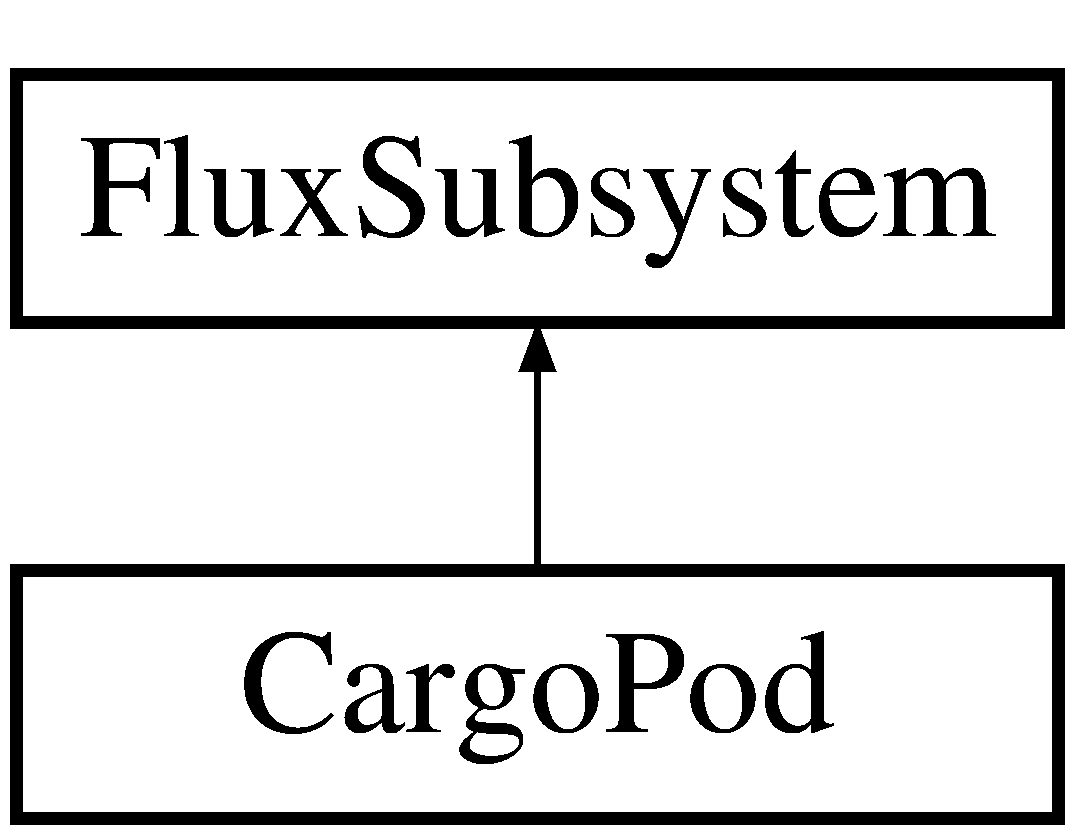
\includegraphics[height=2.000000cm]{classCargoPod}
\end{center}
\end{figure}
\subsection*{Public Member Functions}
\begin{DoxyCompactItemize}
\item 
\hyperlink{classCargoPod_a2c409cfae64e6c554eb7620f5db213d0}{Cargo\+Pod} ()
\item 
void \hyperlink{classCargoPod_a28aaa86f3e7ee713748f4e9b1a136fd8}{robot\+Init} () override
\item 
void \hyperlink{classCargoPod_a22723a1f9685242aca13e6bc44e3f0a2}{robot\+Update} () override
\item 
void \hyperlink{classCargoPod_a2da82d2620414330cd775ac1c7f0718a}{teleop\+Init} () override
\item 
void \hyperlink{classCargoPod_a29fd74f10b26e3db4348e039969fb173}{teleop\+Update} () override
\item 
void \hyperlink{classCargoPod_a070623c3e9ca5b91765d68b63ccfa1eb}{auton\+Init} () override
\item 
void \hyperlink{classCargoPod_ad11b20da5e057212dedd7a5ef34223b9}{auton\+Update} () override
\item 
void \hyperlink{classCargoPod_a924ef514ed33ea4e7f7ef966f5b83fa7}{disabled\+Init} () override
\item 
void \hyperlink{classCargoPod_a71b58a975ba9f20f4a9023aa3fcbba0e}{disabled\+Update} () override
\end{DoxyCompactItemize}


\subsection{Constructor \& Destructor Documentation}
\mbox{\Hypertarget{classCargoPod_a2c409cfae64e6c554eb7620f5db213d0}\label{classCargoPod_a2c409cfae64e6c554eb7620f5db213d0}} 
\index{Cargo\+Pod@{Cargo\+Pod}!Cargo\+Pod@{Cargo\+Pod}}
\index{Cargo\+Pod@{Cargo\+Pod}!Cargo\+Pod@{Cargo\+Pod}}
\subsubsection{\texorpdfstring{Cargo\+Pod()}{CargoPod()}}
{\footnotesize\ttfamily Cargo\+Pod\+::\+Cargo\+Pod (\begin{DoxyParamCaption}{ }\end{DoxyParamCaption})}



\subsection{Member Function Documentation}
\mbox{\Hypertarget{classCargoPod_a070623c3e9ca5b91765d68b63ccfa1eb}\label{classCargoPod_a070623c3e9ca5b91765d68b63ccfa1eb}} 
\index{Cargo\+Pod@{Cargo\+Pod}!auton\+Init@{auton\+Init}}
\index{auton\+Init@{auton\+Init}!Cargo\+Pod@{Cargo\+Pod}}
\subsubsection{\texorpdfstring{auton\+Init()}{autonInit()}}
{\footnotesize\ttfamily void Cargo\+Pod\+::auton\+Init (\begin{DoxyParamCaption}{ }\end{DoxyParamCaption})\hspace{0.3cm}{\ttfamily [override]}, {\ttfamily [virtual]}}



Reimplemented from \hyperlink{classFluxSubsystem_a142cb34f612412e26bd0049e037dbe60}{Flux\+Subsystem}.

\mbox{\Hypertarget{classCargoPod_ad11b20da5e057212dedd7a5ef34223b9}\label{classCargoPod_ad11b20da5e057212dedd7a5ef34223b9}} 
\index{Cargo\+Pod@{Cargo\+Pod}!auton\+Update@{auton\+Update}}
\index{auton\+Update@{auton\+Update}!Cargo\+Pod@{Cargo\+Pod}}
\subsubsection{\texorpdfstring{auton\+Update()}{autonUpdate()}}
{\footnotesize\ttfamily void Cargo\+Pod\+::auton\+Update (\begin{DoxyParamCaption}{ }\end{DoxyParamCaption})\hspace{0.3cm}{\ttfamily [override]}, {\ttfamily [virtual]}}



Reimplemented from \hyperlink{classFluxSubsystem_aceed900af22503022b8d1278f3693f77}{Flux\+Subsystem}.

\mbox{\Hypertarget{classCargoPod_a924ef514ed33ea4e7f7ef966f5b83fa7}\label{classCargoPod_a924ef514ed33ea4e7f7ef966f5b83fa7}} 
\index{Cargo\+Pod@{Cargo\+Pod}!disabled\+Init@{disabled\+Init}}
\index{disabled\+Init@{disabled\+Init}!Cargo\+Pod@{Cargo\+Pod}}
\subsubsection{\texorpdfstring{disabled\+Init()}{disabledInit()}}
{\footnotesize\ttfamily void Cargo\+Pod\+::disabled\+Init (\begin{DoxyParamCaption}{ }\end{DoxyParamCaption})\hspace{0.3cm}{\ttfamily [override]}, {\ttfamily [virtual]}}



Reimplemented from \hyperlink{classFluxSubsystem_aa0b8fde8aa5094627d15d24e545e1da4}{Flux\+Subsystem}.

\mbox{\Hypertarget{classCargoPod_a71b58a975ba9f20f4a9023aa3fcbba0e}\label{classCargoPod_a71b58a975ba9f20f4a9023aa3fcbba0e}} 
\index{Cargo\+Pod@{Cargo\+Pod}!disabled\+Update@{disabled\+Update}}
\index{disabled\+Update@{disabled\+Update}!Cargo\+Pod@{Cargo\+Pod}}
\subsubsection{\texorpdfstring{disabled\+Update()}{disabledUpdate()}}
{\footnotesize\ttfamily void Cargo\+Pod\+::disabled\+Update (\begin{DoxyParamCaption}{ }\end{DoxyParamCaption})\hspace{0.3cm}{\ttfamily [override]}, {\ttfamily [virtual]}}



Reimplemented from \hyperlink{classFluxSubsystem_a5c39cb0f0834cc77a2b8f4f47778da87}{Flux\+Subsystem}.

\mbox{\Hypertarget{classCargoPod_a28aaa86f3e7ee713748f4e9b1a136fd8}\label{classCargoPod_a28aaa86f3e7ee713748f4e9b1a136fd8}} 
\index{Cargo\+Pod@{Cargo\+Pod}!robot\+Init@{robot\+Init}}
\index{robot\+Init@{robot\+Init}!Cargo\+Pod@{Cargo\+Pod}}
\subsubsection{\texorpdfstring{robot\+Init()}{robotInit()}}
{\footnotesize\ttfamily void Cargo\+Pod\+::robot\+Init (\begin{DoxyParamCaption}{ }\end{DoxyParamCaption})\hspace{0.3cm}{\ttfamily [override]}, {\ttfamily [virtual]}}



Reimplemented from \hyperlink{classFluxSubsystem_aacd5ddfcadda0866d5e838de09a60d63}{Flux\+Subsystem}.

\mbox{\Hypertarget{classCargoPod_a22723a1f9685242aca13e6bc44e3f0a2}\label{classCargoPod_a22723a1f9685242aca13e6bc44e3f0a2}} 
\index{Cargo\+Pod@{Cargo\+Pod}!robot\+Update@{robot\+Update}}
\index{robot\+Update@{robot\+Update}!Cargo\+Pod@{Cargo\+Pod}}
\subsubsection{\texorpdfstring{robot\+Update()}{robotUpdate()}}
{\footnotesize\ttfamily void Cargo\+Pod\+::robot\+Update (\begin{DoxyParamCaption}{ }\end{DoxyParamCaption})\hspace{0.3cm}{\ttfamily [override]}, {\ttfamily [virtual]}}



Reimplemented from \hyperlink{classFluxSubsystem_ac2b1c08b53251870e945edf7080c1549}{Flux\+Subsystem}.

\mbox{\Hypertarget{classCargoPod_a2da82d2620414330cd775ac1c7f0718a}\label{classCargoPod_a2da82d2620414330cd775ac1c7f0718a}} 
\index{Cargo\+Pod@{Cargo\+Pod}!teleop\+Init@{teleop\+Init}}
\index{teleop\+Init@{teleop\+Init}!Cargo\+Pod@{Cargo\+Pod}}
\subsubsection{\texorpdfstring{teleop\+Init()}{teleopInit()}}
{\footnotesize\ttfamily void Cargo\+Pod\+::teleop\+Init (\begin{DoxyParamCaption}{ }\end{DoxyParamCaption})\hspace{0.3cm}{\ttfamily [override]}, {\ttfamily [virtual]}}



Reimplemented from \hyperlink{classFluxSubsystem_aec6d05e4f80c3783684598fb92ad2e55}{Flux\+Subsystem}.

\mbox{\Hypertarget{classCargoPod_a29fd74f10b26e3db4348e039969fb173}\label{classCargoPod_a29fd74f10b26e3db4348e039969fb173}} 
\index{Cargo\+Pod@{Cargo\+Pod}!teleop\+Update@{teleop\+Update}}
\index{teleop\+Update@{teleop\+Update}!Cargo\+Pod@{Cargo\+Pod}}
\subsubsection{\texorpdfstring{teleop\+Update()}{teleopUpdate()}}
{\footnotesize\ttfamily void Cargo\+Pod\+::teleop\+Update (\begin{DoxyParamCaption}{ }\end{DoxyParamCaption})\hspace{0.3cm}{\ttfamily [override]}, {\ttfamily [virtual]}}



Reimplemented from \hyperlink{classFluxSubsystem_a327d76affc60699bfa62563e364e42f5}{Flux\+Subsystem}.



The documentation for this class was generated from the following files\+:\begin{DoxyCompactItemize}
\item 
src/main/2019/\+Mechs/\hyperlink{CargoPod_8h}{Cargo\+Pod.\+h}\item 
src/main/2019/\+Mechs/\hyperlink{CargoPod_8cpp}{Cargo\+Pod.\+cpp}\end{DoxyCompactItemize}

\hypertarget{classDatapool}{}\section{Datapool Class Reference}
\label{classDatapool}\index{Datapool@{Datapool}}


{\ttfamily \#include $<$Datapool.\+h$>$}

\subsection*{Public Member Functions}
\begin{DoxyCompactItemize}
\item 
void \hyperlink{classDatapool_afae02fe80bca3b1978317f2f7be8bec1}{Print} ()
\item 
double \hyperlink{classDatapool_a005421262c8c1a71fa93d167492ebb50}{get\+Data} (const std\+::string \&group\+Name, const std\+::string \&sys\+Name)
\item 
void \hyperlink{classDatapool_a4dcd17302657042344f3a1bcefce704f}{add\+Data} (const std\+::string \&group\+Name, const std\+::string \&member\+Name, double value)
\end{DoxyCompactItemize}
\subsection*{Static Public Member Functions}
\begin{DoxyCompactItemize}
\item 
static \hyperlink{classDatapool}{Datapool} \& \hyperlink{classDatapool_a9cfbb881291c80d851d0df66341b6299}{get\+Instance} ()
\end{DoxyCompactItemize}


\subsection{Detailed Description}
Singleton that allows to share info between subsystems, currently relies solely on a string double k v pair 

\subsection{Member Function Documentation}
\mbox{\Hypertarget{classDatapool_a4dcd17302657042344f3a1bcefce704f}\label{classDatapool_a4dcd17302657042344f3a1bcefce704f}} 
\index{Datapool@{Datapool}!add\+Data@{add\+Data}}
\index{add\+Data@{add\+Data}!Datapool@{Datapool}}
\subsubsection{\texorpdfstring{add\+Data()}{addData()}}
{\footnotesize\ttfamily void Datapool\+::add\+Data (\begin{DoxyParamCaption}\item[{const std\+::string \&}]{group\+Name,  }\item[{const std\+::string \&}]{member\+Name,  }\item[{double}]{value }\end{DoxyParamCaption})}

Requires a groupname to avoid overwritting another map \mbox{\Hypertarget{classDatapool_a005421262c8c1a71fa93d167492ebb50}\label{classDatapool_a005421262c8c1a71fa93d167492ebb50}} 
\index{Datapool@{Datapool}!get\+Data@{get\+Data}}
\index{get\+Data@{get\+Data}!Datapool@{Datapool}}
\subsubsection{\texorpdfstring{get\+Data()}{getData()}}
{\footnotesize\ttfamily double Datapool\+::get\+Data (\begin{DoxyParamCaption}\item[{const std\+::string \&}]{group\+Name,  }\item[{const std\+::string \&}]{member\+Name }\end{DoxyParamCaption})}

Accessing data requires a groupname entry, returns saved double value \mbox{\Hypertarget{classDatapool_a9cfbb881291c80d851d0df66341b6299}\label{classDatapool_a9cfbb881291c80d851d0df66341b6299}} 
\index{Datapool@{Datapool}!get\+Instance@{get\+Instance}}
\index{get\+Instance@{get\+Instance}!Datapool@{Datapool}}
\subsubsection{\texorpdfstring{get\+Instance()}{getInstance()}}
{\footnotesize\ttfamily \hyperlink{classDatapool}{Datapool} \& Datapool\+::get\+Instance (\begin{DoxyParamCaption}{ }\end{DoxyParamCaption})\hspace{0.3cm}{\ttfamily [static]}}

\mbox{\Hypertarget{classDatapool_afae02fe80bca3b1978317f2f7be8bec1}\label{classDatapool_afae02fe80bca3b1978317f2f7be8bec1}} 
\index{Datapool@{Datapool}!Print@{Print}}
\index{Print@{Print}!Datapool@{Datapool}}
\subsubsection{\texorpdfstring{Print()}{Print()}}
{\footnotesize\ttfamily void Datapool\+::\+Print (\begin{DoxyParamCaption}{ }\end{DoxyParamCaption})}



The documentation for this class was generated from the following files\+:\begin{DoxyCompactItemize}
\item 
src/main/\+Subsystems/\hyperlink{Datapool_8h}{Datapool.\+h}\item 
src/main/\+Subsystems/\hyperlink{Datapool_8cpp}{Datapool.\+cpp}\end{DoxyCompactItemize}

\hypertarget{classDelorean}{}\section{Delorean Class Reference}
\label{classDelorean}\index{Delorean@{Delorean}}


{\ttfamily \#include $<$Delorean.\+h$>$}

Inheritance diagram for Delorean\+:\begin{figure}[H]
\begin{center}
\leavevmode
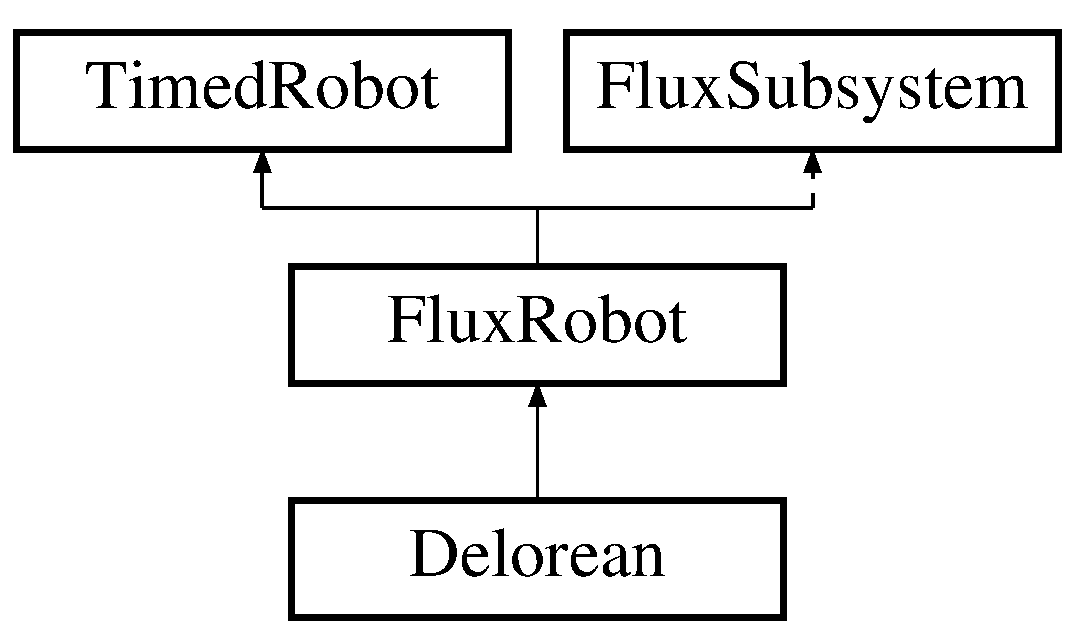
\includegraphics[height=3.000000cm]{classDelorean}
\end{center}
\end{figure}
\subsection*{Public Member Functions}
\begin{DoxyCompactItemize}
\item 
\hyperlink{classDelorean_a80afc6fe9ba8edac0af62189b8afbbd3}{Delorean} ()
\item 
void \hyperlink{classDelorean_a2baeb249408fd1d61da69b1edd832554}{add\+Properties} () override
\item 
void \hyperlink{classDelorean_a8ccfc53654ee0512a7e6ba1d6ba739c0}{init\+Subsystems} () override
\item 
void \hyperlink{classDelorean_a591e1b68a21a82c7e1cf4e7dbf5294a2}{robot\+Init} () override
\item 
void \hyperlink{classDelorean_a47b9cfdb59a6f46ee26f45f794e313c1}{robot\+Update} () override
\item 
void \hyperlink{classDelorean_a789c6e4e70f4e2cfdf944d1a1a149509}{teleop\+Init} () override
\item 
void \hyperlink{classDelorean_a6053dfc106d71fcffa30bac0f5e9b5b8}{teleop\+Update} () override
\item 
void \hyperlink{classDelorean_ad06990e5c59d5f4d30b48015e744cc49}{auton\+Init} () override
\item 
void \hyperlink{classDelorean_a17c9b875c9c0d3c9b9dadd5838bfedfd}{auton\+Update} () override
\item 
void \hyperlink{classDelorean_ae054ba79b38b46d20e50becb5d31884c}{disabled\+Init} () override
\item 
void \hyperlink{classDelorean_acc8f7d93dd894233d16f34316d363983}{disabled\+Update} () override
\end{DoxyCompactItemize}
\subsection*{Additional Inherited Members}


\subsection{Constructor \& Destructor Documentation}
\mbox{\Hypertarget{classDelorean_a80afc6fe9ba8edac0af62189b8afbbd3}\label{classDelorean_a80afc6fe9ba8edac0af62189b8afbbd3}} 
\index{Delorean@{Delorean}!Delorean@{Delorean}}
\index{Delorean@{Delorean}!Delorean@{Delorean}}
\subsubsection{\texorpdfstring{Delorean()}{Delorean()}}
{\footnotesize\ttfamily Delorean\+::\+Delorean (\begin{DoxyParamCaption}{ }\end{DoxyParamCaption})}



\subsection{Member Function Documentation}
\mbox{\Hypertarget{classDelorean_a2baeb249408fd1d61da69b1edd832554}\label{classDelorean_a2baeb249408fd1d61da69b1edd832554}} 
\index{Delorean@{Delorean}!add\+Properties@{add\+Properties}}
\index{add\+Properties@{add\+Properties}!Delorean@{Delorean}}
\subsubsection{\texorpdfstring{add\+Properties()}{addProperties()}}
{\footnotesize\ttfamily void Delorean\+::add\+Properties (\begin{DoxyParamCaption}{ }\end{DoxyParamCaption})\hspace{0.3cm}{\ttfamily [override]}, {\ttfamily [virtual]}}



Implements \hyperlink{classFluxRobot_a6f7940d8f82e80a6e405bad20ec9a5a5}{Flux\+Robot}.

\mbox{\Hypertarget{classDelorean_ad06990e5c59d5f4d30b48015e744cc49}\label{classDelorean_ad06990e5c59d5f4d30b48015e744cc49}} 
\index{Delorean@{Delorean}!auton\+Init@{auton\+Init}}
\index{auton\+Init@{auton\+Init}!Delorean@{Delorean}}
\subsubsection{\texorpdfstring{auton\+Init()}{autonInit()}}
{\footnotesize\ttfamily void Delorean\+::auton\+Init (\begin{DoxyParamCaption}{ }\end{DoxyParamCaption})\hspace{0.3cm}{\ttfamily [override]}, {\ttfamily [virtual]}}



Reimplemented from \hyperlink{classFluxSubsystem_a142cb34f612412e26bd0049e037dbe60}{Flux\+Subsystem}.

\mbox{\Hypertarget{classDelorean_a17c9b875c9c0d3c9b9dadd5838bfedfd}\label{classDelorean_a17c9b875c9c0d3c9b9dadd5838bfedfd}} 
\index{Delorean@{Delorean}!auton\+Update@{auton\+Update}}
\index{auton\+Update@{auton\+Update}!Delorean@{Delorean}}
\subsubsection{\texorpdfstring{auton\+Update()}{autonUpdate()}}
{\footnotesize\ttfamily void Delorean\+::auton\+Update (\begin{DoxyParamCaption}{ }\end{DoxyParamCaption})\hspace{0.3cm}{\ttfamily [override]}, {\ttfamily [virtual]}}



Reimplemented from \hyperlink{classFluxSubsystem_aceed900af22503022b8d1278f3693f77}{Flux\+Subsystem}.

\mbox{\Hypertarget{classDelorean_ae054ba79b38b46d20e50becb5d31884c}\label{classDelorean_ae054ba79b38b46d20e50becb5d31884c}} 
\index{Delorean@{Delorean}!disabled\+Init@{disabled\+Init}}
\index{disabled\+Init@{disabled\+Init}!Delorean@{Delorean}}
\subsubsection{\texorpdfstring{disabled\+Init()}{disabledInit()}}
{\footnotesize\ttfamily void Delorean\+::disabled\+Init (\begin{DoxyParamCaption}{ }\end{DoxyParamCaption})\hspace{0.3cm}{\ttfamily [override]}, {\ttfamily [virtual]}}



Reimplemented from \hyperlink{classFluxSubsystem_aa0b8fde8aa5094627d15d24e545e1da4}{Flux\+Subsystem}.

\mbox{\Hypertarget{classDelorean_acc8f7d93dd894233d16f34316d363983}\label{classDelorean_acc8f7d93dd894233d16f34316d363983}} 
\index{Delorean@{Delorean}!disabled\+Update@{disabled\+Update}}
\index{disabled\+Update@{disabled\+Update}!Delorean@{Delorean}}
\subsubsection{\texorpdfstring{disabled\+Update()}{disabledUpdate()}}
{\footnotesize\ttfamily void Delorean\+::disabled\+Update (\begin{DoxyParamCaption}{ }\end{DoxyParamCaption})\hspace{0.3cm}{\ttfamily [override]}, {\ttfamily [virtual]}}



Reimplemented from \hyperlink{classFluxSubsystem_a5c39cb0f0834cc77a2b8f4f47778da87}{Flux\+Subsystem}.

\mbox{\Hypertarget{classDelorean_a8ccfc53654ee0512a7e6ba1d6ba739c0}\label{classDelorean_a8ccfc53654ee0512a7e6ba1d6ba739c0}} 
\index{Delorean@{Delorean}!init\+Subsystems@{init\+Subsystems}}
\index{init\+Subsystems@{init\+Subsystems}!Delorean@{Delorean}}
\subsubsection{\texorpdfstring{init\+Subsystems()}{initSubsystems()}}
{\footnotesize\ttfamily void Delorean\+::init\+Subsystems (\begin{DoxyParamCaption}{ }\end{DoxyParamCaption})\hspace{0.3cm}{\ttfamily [override]}, {\ttfamily [virtual]}}

Add subsystems here 

Implements \hyperlink{classFluxRobot_aa5fcf98b4dfd539b1b49772381578dc8}{Flux\+Robot}.

\mbox{\Hypertarget{classDelorean_a591e1b68a21a82c7e1cf4e7dbf5294a2}\label{classDelorean_a591e1b68a21a82c7e1cf4e7dbf5294a2}} 
\index{Delorean@{Delorean}!robot\+Init@{robot\+Init}}
\index{robot\+Init@{robot\+Init}!Delorean@{Delorean}}
\subsubsection{\texorpdfstring{robot\+Init()}{robotInit()}}
{\footnotesize\ttfamily void Delorean\+::robot\+Init (\begin{DoxyParamCaption}{ }\end{DoxyParamCaption})\hspace{0.3cm}{\ttfamily [override]}, {\ttfamily [virtual]}}



Reimplemented from \hyperlink{classFluxSubsystem_aacd5ddfcadda0866d5e838de09a60d63}{Flux\+Subsystem}.

\mbox{\Hypertarget{classDelorean_a47b9cfdb59a6f46ee26f45f794e313c1}\label{classDelorean_a47b9cfdb59a6f46ee26f45f794e313c1}} 
\index{Delorean@{Delorean}!robot\+Update@{robot\+Update}}
\index{robot\+Update@{robot\+Update}!Delorean@{Delorean}}
\subsubsection{\texorpdfstring{robot\+Update()}{robotUpdate()}}
{\footnotesize\ttfamily void Delorean\+::robot\+Update (\begin{DoxyParamCaption}{ }\end{DoxyParamCaption})\hspace{0.3cm}{\ttfamily [override]}, {\ttfamily [virtual]}}



Reimplemented from \hyperlink{classFluxSubsystem_ac2b1c08b53251870e945edf7080c1549}{Flux\+Subsystem}.

\mbox{\Hypertarget{classDelorean_a789c6e4e70f4e2cfdf944d1a1a149509}\label{classDelorean_a789c6e4e70f4e2cfdf944d1a1a149509}} 
\index{Delorean@{Delorean}!teleop\+Init@{teleop\+Init}}
\index{teleop\+Init@{teleop\+Init}!Delorean@{Delorean}}
\subsubsection{\texorpdfstring{teleop\+Init()}{teleopInit()}}
{\footnotesize\ttfamily void Delorean\+::teleop\+Init (\begin{DoxyParamCaption}{ }\end{DoxyParamCaption})\hspace{0.3cm}{\ttfamily [override]}, {\ttfamily [virtual]}}



Reimplemented from \hyperlink{classFluxSubsystem_aec6d05e4f80c3783684598fb92ad2e55}{Flux\+Subsystem}.

\mbox{\Hypertarget{classDelorean_a6053dfc106d71fcffa30bac0f5e9b5b8}\label{classDelorean_a6053dfc106d71fcffa30bac0f5e9b5b8}} 
\index{Delorean@{Delorean}!teleop\+Update@{teleop\+Update}}
\index{teleop\+Update@{teleop\+Update}!Delorean@{Delorean}}
\subsubsection{\texorpdfstring{teleop\+Update()}{teleopUpdate()}}
{\footnotesize\ttfamily void Delorean\+::teleop\+Update (\begin{DoxyParamCaption}{ }\end{DoxyParamCaption})\hspace{0.3cm}{\ttfamily [override]}, {\ttfamily [virtual]}}



Reimplemented from \hyperlink{classFluxSubsystem_a327d76affc60699bfa62563e364e42f5}{Flux\+Subsystem}.



The documentation for this class was generated from the following files\+:\begin{DoxyCompactItemize}
\item 
src/main/2019/\+Robots/\hyperlink{Delorean_8h}{Delorean.\+h}\item 
src/main/2019/\+Robots/\hyperlink{Delorean_8cpp}{Delorean.\+cpp}\end{DoxyCompactItemize}

\hypertarget{classDrivetrain}{}\section{Drivetrain Class Reference}
\label{classDrivetrain}\index{Drivetrain@{Drivetrain}}


{\ttfamily \#include $<$Drive\+Train.\+h$>$}

Inheritance diagram for Drivetrain\+:\begin{figure}[H]
\begin{center}
\leavevmode
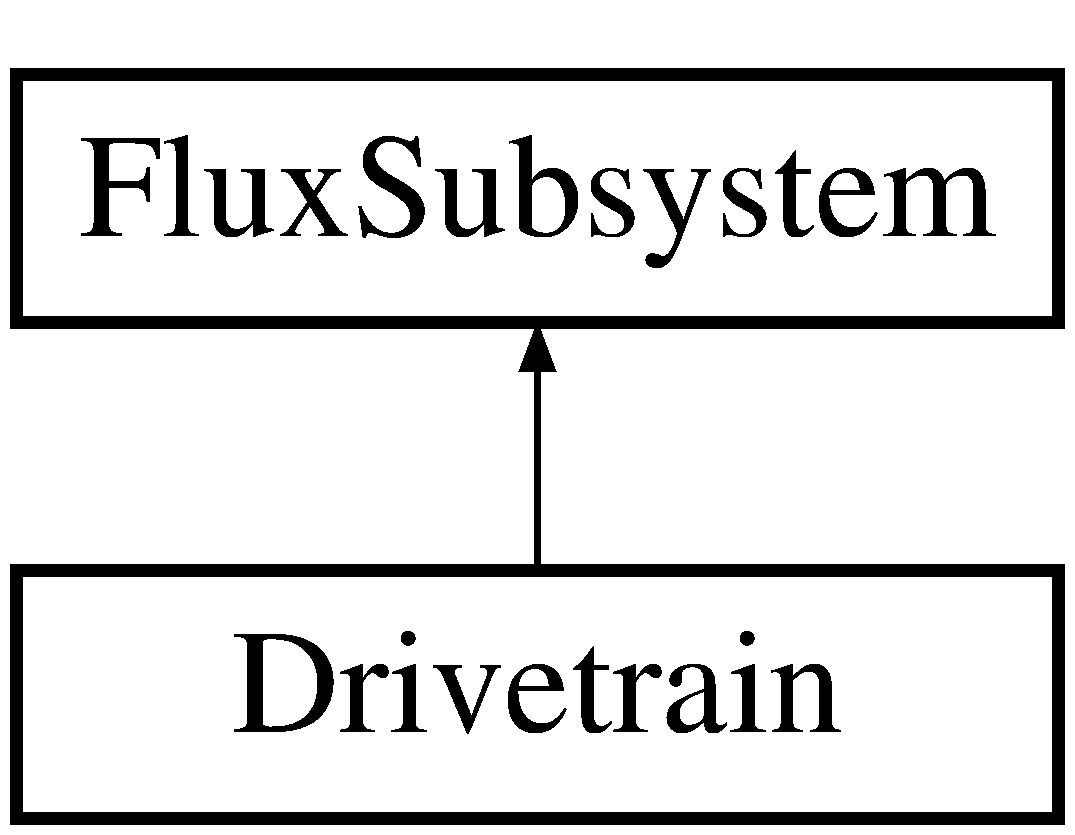
\includegraphics[height=2.000000cm]{classDrivetrain}
\end{center}
\end{figure}
\subsection*{Public Member Functions}
\begin{DoxyCompactItemize}
\item 
\hyperlink{classDrivetrain_abfcc3eea7516b5f76422d39676adbd27}{Drivetrain} ()
\item 
void \hyperlink{classDrivetrain_a7e9c10a27b3cc5ad89f2338de39b7c62}{robot\+Init} () override
\item 
void \hyperlink{classDrivetrain_a2a2b5976426dc0c1f45438fd7a5926e4}{robot\+Update} () override
\item 
void \hyperlink{classDrivetrain_a12d7edbb3a1b5d4ffa4ecb381c1ab115}{teleop\+Init} () override
\item 
void \hyperlink{classDrivetrain_a3b6bdf96a9388285c7560b2fedfc7ca1}{teleop\+Update} () override
\item 
void \hyperlink{classDrivetrain_a6aec7fa1a9daf1233a59fe0243d3bc8c}{auton\+Init} () override
\item 
void \hyperlink{classDrivetrain_ab451b48c598fa715ff1a8117ddc6f705}{auton\+Update} () override
\item 
void \hyperlink{classDrivetrain_ac6fe041de609bdb45eac65282fbdf507}{disabled\+Init} () override
\item 
void \hyperlink{classDrivetrain_a46aa479a25757868bfda71081ec7baa2}{disabled\+Update} () override
\end{DoxyCompactItemize}


\subsection{Constructor \& Destructor Documentation}
\mbox{\Hypertarget{classDrivetrain_abfcc3eea7516b5f76422d39676adbd27}\label{classDrivetrain_abfcc3eea7516b5f76422d39676adbd27}} 
\index{Drivetrain@{Drivetrain}!Drivetrain@{Drivetrain}}
\index{Drivetrain@{Drivetrain}!Drivetrain@{Drivetrain}}
\subsubsection{\texorpdfstring{Drivetrain()}{Drivetrain()}}
{\footnotesize\ttfamily Drivetrain\+::\+Drivetrain (\begin{DoxyParamCaption}{ }\end{DoxyParamCaption})}



\subsection{Member Function Documentation}
\mbox{\Hypertarget{classDrivetrain_a6aec7fa1a9daf1233a59fe0243d3bc8c}\label{classDrivetrain_a6aec7fa1a9daf1233a59fe0243d3bc8c}} 
\index{Drivetrain@{Drivetrain}!auton\+Init@{auton\+Init}}
\index{auton\+Init@{auton\+Init}!Drivetrain@{Drivetrain}}
\subsubsection{\texorpdfstring{auton\+Init()}{autonInit()}}
{\footnotesize\ttfamily void Drivetrain\+::auton\+Init (\begin{DoxyParamCaption}{ }\end{DoxyParamCaption})\hspace{0.3cm}{\ttfamily [override]}, {\ttfamily [virtual]}}



Reimplemented from \hyperlink{classFluxSubsystem_a142cb34f612412e26bd0049e037dbe60}{Flux\+Subsystem}.

\mbox{\Hypertarget{classDrivetrain_ab451b48c598fa715ff1a8117ddc6f705}\label{classDrivetrain_ab451b48c598fa715ff1a8117ddc6f705}} 
\index{Drivetrain@{Drivetrain}!auton\+Update@{auton\+Update}}
\index{auton\+Update@{auton\+Update}!Drivetrain@{Drivetrain}}
\subsubsection{\texorpdfstring{auton\+Update()}{autonUpdate()}}
{\footnotesize\ttfamily void Drivetrain\+::auton\+Update (\begin{DoxyParamCaption}{ }\end{DoxyParamCaption})\hspace{0.3cm}{\ttfamily [override]}, {\ttfamily [virtual]}}



Reimplemented from \hyperlink{classFluxSubsystem_aceed900af22503022b8d1278f3693f77}{Flux\+Subsystem}.

\mbox{\Hypertarget{classDrivetrain_ac6fe041de609bdb45eac65282fbdf507}\label{classDrivetrain_ac6fe041de609bdb45eac65282fbdf507}} 
\index{Drivetrain@{Drivetrain}!disabled\+Init@{disabled\+Init}}
\index{disabled\+Init@{disabled\+Init}!Drivetrain@{Drivetrain}}
\subsubsection{\texorpdfstring{disabled\+Init()}{disabledInit()}}
{\footnotesize\ttfamily void Drivetrain\+::disabled\+Init (\begin{DoxyParamCaption}{ }\end{DoxyParamCaption})\hspace{0.3cm}{\ttfamily [override]}, {\ttfamily [virtual]}}



Reimplemented from \hyperlink{classFluxSubsystem_aa0b8fde8aa5094627d15d24e545e1da4}{Flux\+Subsystem}.

\mbox{\Hypertarget{classDrivetrain_a46aa479a25757868bfda71081ec7baa2}\label{classDrivetrain_a46aa479a25757868bfda71081ec7baa2}} 
\index{Drivetrain@{Drivetrain}!disabled\+Update@{disabled\+Update}}
\index{disabled\+Update@{disabled\+Update}!Drivetrain@{Drivetrain}}
\subsubsection{\texorpdfstring{disabled\+Update()}{disabledUpdate()}}
{\footnotesize\ttfamily void Drivetrain\+::disabled\+Update (\begin{DoxyParamCaption}{ }\end{DoxyParamCaption})\hspace{0.3cm}{\ttfamily [override]}, {\ttfamily [virtual]}}



Reimplemented from \hyperlink{classFluxSubsystem_a5c39cb0f0834cc77a2b8f4f47778da87}{Flux\+Subsystem}.

\mbox{\Hypertarget{classDrivetrain_a7e9c10a27b3cc5ad89f2338de39b7c62}\label{classDrivetrain_a7e9c10a27b3cc5ad89f2338de39b7c62}} 
\index{Drivetrain@{Drivetrain}!robot\+Init@{robot\+Init}}
\index{robot\+Init@{robot\+Init}!Drivetrain@{Drivetrain}}
\subsubsection{\texorpdfstring{robot\+Init()}{robotInit()}}
{\footnotesize\ttfamily void Drivetrain\+::robot\+Init (\begin{DoxyParamCaption}{ }\end{DoxyParamCaption})\hspace{0.3cm}{\ttfamily [override]}, {\ttfamily [virtual]}}



Reimplemented from \hyperlink{classFluxSubsystem_aacd5ddfcadda0866d5e838de09a60d63}{Flux\+Subsystem}.

\mbox{\Hypertarget{classDrivetrain_a2a2b5976426dc0c1f45438fd7a5926e4}\label{classDrivetrain_a2a2b5976426dc0c1f45438fd7a5926e4}} 
\index{Drivetrain@{Drivetrain}!robot\+Update@{robot\+Update}}
\index{robot\+Update@{robot\+Update}!Drivetrain@{Drivetrain}}
\subsubsection{\texorpdfstring{robot\+Update()}{robotUpdate()}}
{\footnotesize\ttfamily void Drivetrain\+::robot\+Update (\begin{DoxyParamCaption}{ }\end{DoxyParamCaption})\hspace{0.3cm}{\ttfamily [override]}, {\ttfamily [virtual]}}



Reimplemented from \hyperlink{classFluxSubsystem_ac2b1c08b53251870e945edf7080c1549}{Flux\+Subsystem}.

\mbox{\Hypertarget{classDrivetrain_a12d7edbb3a1b5d4ffa4ecb381c1ab115}\label{classDrivetrain_a12d7edbb3a1b5d4ffa4ecb381c1ab115}} 
\index{Drivetrain@{Drivetrain}!teleop\+Init@{teleop\+Init}}
\index{teleop\+Init@{teleop\+Init}!Drivetrain@{Drivetrain}}
\subsubsection{\texorpdfstring{teleop\+Init()}{teleopInit()}}
{\footnotesize\ttfamily void Drivetrain\+::teleop\+Init (\begin{DoxyParamCaption}{ }\end{DoxyParamCaption})\hspace{0.3cm}{\ttfamily [override]}, {\ttfamily [virtual]}}



Reimplemented from \hyperlink{classFluxSubsystem_aec6d05e4f80c3783684598fb92ad2e55}{Flux\+Subsystem}.

\mbox{\Hypertarget{classDrivetrain_a3b6bdf96a9388285c7560b2fedfc7ca1}\label{classDrivetrain_a3b6bdf96a9388285c7560b2fedfc7ca1}} 
\index{Drivetrain@{Drivetrain}!teleop\+Update@{teleop\+Update}}
\index{teleop\+Update@{teleop\+Update}!Drivetrain@{Drivetrain}}
\subsubsection{\texorpdfstring{teleop\+Update()}{teleopUpdate()}}
{\footnotesize\ttfamily void Drivetrain\+::teleop\+Update (\begin{DoxyParamCaption}{ }\end{DoxyParamCaption})\hspace{0.3cm}{\ttfamily [override]}, {\ttfamily [virtual]}}



Reimplemented from \hyperlink{classFluxSubsystem_a327d76affc60699bfa62563e364e42f5}{Flux\+Subsystem}.



The documentation for this class was generated from the following files\+:\begin{DoxyCompactItemize}
\item 
src/main/2019/\+Mechs/\hyperlink{DriveTrain_8h}{Drive\+Train.\+h}\item 
src/main/2019/\+Mechs/\hyperlink{DriveTrain_8cpp}{Drive\+Train.\+cpp}\end{DoxyCompactItemize}

\hypertarget{classFluxcontroller}{}\section{Fluxcontroller Class Reference}
\label{classFluxcontroller}\index{Fluxcontroller@{Fluxcontroller}}


{\ttfamily \#include $<$Flux\+Controller.\+h$>$}

Inheritance diagram for Fluxcontroller\+:\begin{figure}[H]
\begin{center}
\leavevmode
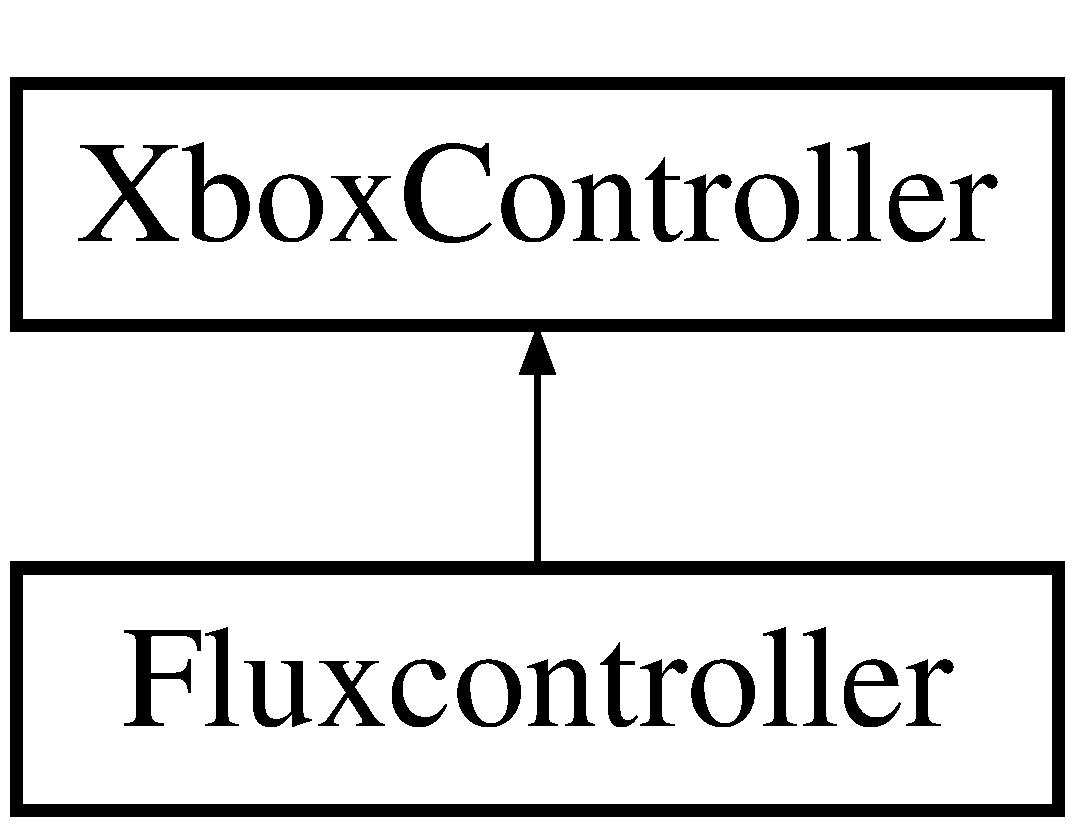
\includegraphics[height=2.000000cm]{classFluxcontroller}
\end{center}
\end{figure}
\subsection*{Public Member Functions}
\begin{DoxyCompactItemize}
\item 
\hyperlink{classFluxcontroller_a1451c531fa6e91f5a1a34b7d06286846}{Fluxcontroller} (unsigned int U\+S\+B\+Port)
\item 
double \hyperlink{classFluxcontroller_ab3801948ee5152689b8d8e8ac6e92856}{joystick} (Generic\+H\+I\+D\+::\+Joystick\+Hand)
\item 
void \hyperlink{classFluxcontroller_a82147680c873b1da821dfb48a38f0b9a}{set\+Exp\+Joystick} (bool input)
\item 
void \hyperlink{classFluxcontroller_ac2d888be1a50f85ccbae685171d5359f}{negate} (bool input)
\end{DoxyCompactItemize}


\subsection{Detailed Description}
This class adds some overture goodies to input mode 

\subsection{Constructor \& Destructor Documentation}
\mbox{\Hypertarget{classFluxcontroller_a1451c531fa6e91f5a1a34b7d06286846}\label{classFluxcontroller_a1451c531fa6e91f5a1a34b7d06286846}} 
\index{Fluxcontroller@{Fluxcontroller}!Fluxcontroller@{Fluxcontroller}}
\index{Fluxcontroller@{Fluxcontroller}!Fluxcontroller@{Fluxcontroller}}
\subsubsection{\texorpdfstring{Fluxcontroller()}{Fluxcontroller()}}
{\footnotesize\ttfamily Fluxcontroller\+::\+Fluxcontroller (\begin{DoxyParamCaption}\item[{unsigned int}]{U\+S\+B\+Port }\end{DoxyParamCaption})}



\subsection{Member Function Documentation}
\mbox{\Hypertarget{classFluxcontroller_ab3801948ee5152689b8d8e8ac6e92856}\label{classFluxcontroller_ab3801948ee5152689b8d8e8ac6e92856}} 
\index{Fluxcontroller@{Fluxcontroller}!joystick@{joystick}}
\index{joystick@{joystick}!Fluxcontroller@{Fluxcontroller}}
\subsubsection{\texorpdfstring{joystick()}{joystick()}}
{\footnotesize\ttfamily double Fluxcontroller\+::joystick (\begin{DoxyParamCaption}\item[{Generic\+H\+I\+D\+::\+Joystick\+Hand}]{hand }\end{DoxyParamCaption})}

\mbox{\Hypertarget{classFluxcontroller_ac2d888be1a50f85ccbae685171d5359f}\label{classFluxcontroller_ac2d888be1a50f85ccbae685171d5359f}} 
\index{Fluxcontroller@{Fluxcontroller}!negate@{negate}}
\index{negate@{negate}!Fluxcontroller@{Fluxcontroller}}
\subsubsection{\texorpdfstring{negate()}{negate()}}
{\footnotesize\ttfamily void Fluxcontroller\+::negate (\begin{DoxyParamCaption}\item[{bool}]{input }\end{DoxyParamCaption})}

\mbox{\Hypertarget{classFluxcontroller_a82147680c873b1da821dfb48a38f0b9a}\label{classFluxcontroller_a82147680c873b1da821dfb48a38f0b9a}} 
\index{Fluxcontroller@{Fluxcontroller}!set\+Exp\+Joystick@{set\+Exp\+Joystick}}
\index{set\+Exp\+Joystick@{set\+Exp\+Joystick}!Fluxcontroller@{Fluxcontroller}}
\subsubsection{\texorpdfstring{set\+Exp\+Joystick()}{setExpJoystick()}}
{\footnotesize\ttfamily void Fluxcontroller\+::set\+Exp\+Joystick (\begin{DoxyParamCaption}\item[{bool}]{input }\end{DoxyParamCaption})}



The documentation for this class was generated from the following files\+:\begin{DoxyCompactItemize}
\item 
src/main/\+Utilities/\hyperlink{FluxController_8h}{Flux\+Controller.\+h}\item 
src/main/\+Utilities/\hyperlink{FluxController_8cpp}{Flux\+Controller.\+cpp}\end{DoxyCompactItemize}

\hypertarget{classFluxRobot}{}\section{Flux\+Robot Class Reference}
\label{classFluxRobot}\index{Flux\+Robot@{Flux\+Robot}}


{\ttfamily \#include $<$Flux\+Robot.\+h$>$}

Inheritance diagram for Flux\+Robot\+:\begin{figure}[H]
\begin{center}
\leavevmode
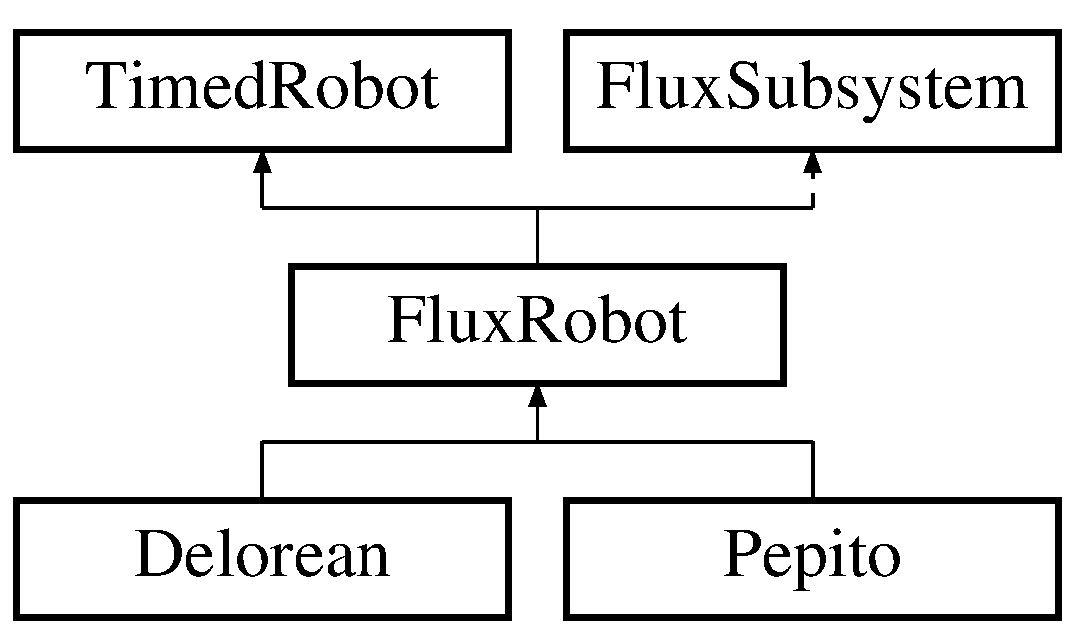
\includegraphics[height=3.000000cm]{classFluxRobot}
\end{center}
\end{figure}
\subsection*{Public Member Functions}
\begin{DoxyCompactItemize}
\item 
\hyperlink{classFluxRobot_aaf20a889c03907de208317746f733d7a}{Flux\+Robot} (const std\+::string \&robot\+Name)
\item 
virtual void \hyperlink{classFluxRobot_aa5fcf98b4dfd539b1b49772381578dc8}{init\+Subsystems} ()=0
\item 
virtual void \hyperlink{classFluxRobot_a6f7940d8f82e80a6e405bad20ec9a5a5}{add\+Properties} ()=0
\end{DoxyCompactItemize}
\subsection*{Protected Attributes}
\begin{DoxyCompactItemize}
\item 
\hyperlink{classSubsystemManager}{Subsystem\+Manager} \& \hyperlink{classFluxRobot_a55d2406f800dddb8f7d4754ef5fb2ede}{manager} = \hyperlink{classSubsystemManager_a3acce674e15d2534ed8a0877b78ac64d}{Subsystem\+Manager\+::get\+Instance}()
\end{DoxyCompactItemize}
\subsection*{Additional Inherited Members}


\subsection{Constructor \& Destructor Documentation}
\mbox{\Hypertarget{classFluxRobot_aaf20a889c03907de208317746f733d7a}\label{classFluxRobot_aaf20a889c03907de208317746f733d7a}} 
\index{Flux\+Robot@{Flux\+Robot}!Flux\+Robot@{Flux\+Robot}}
\index{Flux\+Robot@{Flux\+Robot}!Flux\+Robot@{Flux\+Robot}}
\subsubsection{\texorpdfstring{Flux\+Robot()}{FluxRobot()}}
{\footnotesize\ttfamily Flux\+Robot\+::\+Flux\+Robot (\begin{DoxyParamCaption}\item[{const std\+::string \&}]{robot\+Name }\end{DoxyParamCaption})\hspace{0.3cm}{\ttfamily [explicit]}}



\subsection{Member Function Documentation}
\mbox{\Hypertarget{classFluxRobot_a6f7940d8f82e80a6e405bad20ec9a5a5}\label{classFluxRobot_a6f7940d8f82e80a6e405bad20ec9a5a5}} 
\index{Flux\+Robot@{Flux\+Robot}!add\+Properties@{add\+Properties}}
\index{add\+Properties@{add\+Properties}!Flux\+Robot@{Flux\+Robot}}
\subsubsection{\texorpdfstring{add\+Properties()}{addProperties()}}
{\footnotesize\ttfamily virtual void Flux\+Robot\+::add\+Properties (\begin{DoxyParamCaption}{ }\end{DoxyParamCaption})\hspace{0.3cm}{\ttfamily [pure virtual]}}



Implemented in \hyperlink{classPepito_a1368f048f197d9b0e3a7e710dd4809fc}{Pepito}, and \hyperlink{classDelorean_a2baeb249408fd1d61da69b1edd832554}{Delorean}.

\mbox{\Hypertarget{classFluxRobot_aa5fcf98b4dfd539b1b49772381578dc8}\label{classFluxRobot_aa5fcf98b4dfd539b1b49772381578dc8}} 
\index{Flux\+Robot@{Flux\+Robot}!init\+Subsystems@{init\+Subsystems}}
\index{init\+Subsystems@{init\+Subsystems}!Flux\+Robot@{Flux\+Robot}}
\subsubsection{\texorpdfstring{init\+Subsystems()}{initSubsystems()}}
{\footnotesize\ttfamily virtual void Flux\+Robot\+::init\+Subsystems (\begin{DoxyParamCaption}{ }\end{DoxyParamCaption})\hspace{0.3cm}{\ttfamily [pure virtual]}}

Add subsystems here 

Implemented in \hyperlink{classPepito_a420a3322a1fa658e9e40f277e7cc1c03}{Pepito}, and \hyperlink{classDelorean_a8ccfc53654ee0512a7e6ba1d6ba739c0}{Delorean}.



\subsection{Member Data Documentation}
\mbox{\Hypertarget{classFluxRobot_a55d2406f800dddb8f7d4754ef5fb2ede}\label{classFluxRobot_a55d2406f800dddb8f7d4754ef5fb2ede}} 
\index{Flux\+Robot@{Flux\+Robot}!manager@{manager}}
\index{manager@{manager}!Flux\+Robot@{Flux\+Robot}}
\subsubsection{\texorpdfstring{manager}{manager}}
{\footnotesize\ttfamily \hyperlink{classSubsystemManager}{Subsystem\+Manager}\& Flux\+Robot\+::manager = \hyperlink{classSubsystemManager_a3acce674e15d2534ed8a0877b78ac64d}{Subsystem\+Manager\+::get\+Instance}()\hspace{0.3cm}{\ttfamily [protected]}}



The documentation for this class was generated from the following files\+:\begin{DoxyCompactItemize}
\item 
src/main/\+Subsystems/\hyperlink{FluxRobot_8h}{Flux\+Robot.\+h}\item 
src/main/\+Subsystems/\hyperlink{FluxRobot_8cpp}{Flux\+Robot.\+cpp}\end{DoxyCompactItemize}

\hypertarget{classFluxRS450}{}\section{Flux\+R\+S450 Class Reference}
\label{classFluxRS450}\index{Flux\+R\+S450@{Flux\+R\+S450}}


{\ttfamily \#include $<$Flux\+R\+S450.\+h$>$}

Inheritance diagram for Flux\+R\+S450\+:\begin{figure}[H]
\begin{center}
\leavevmode
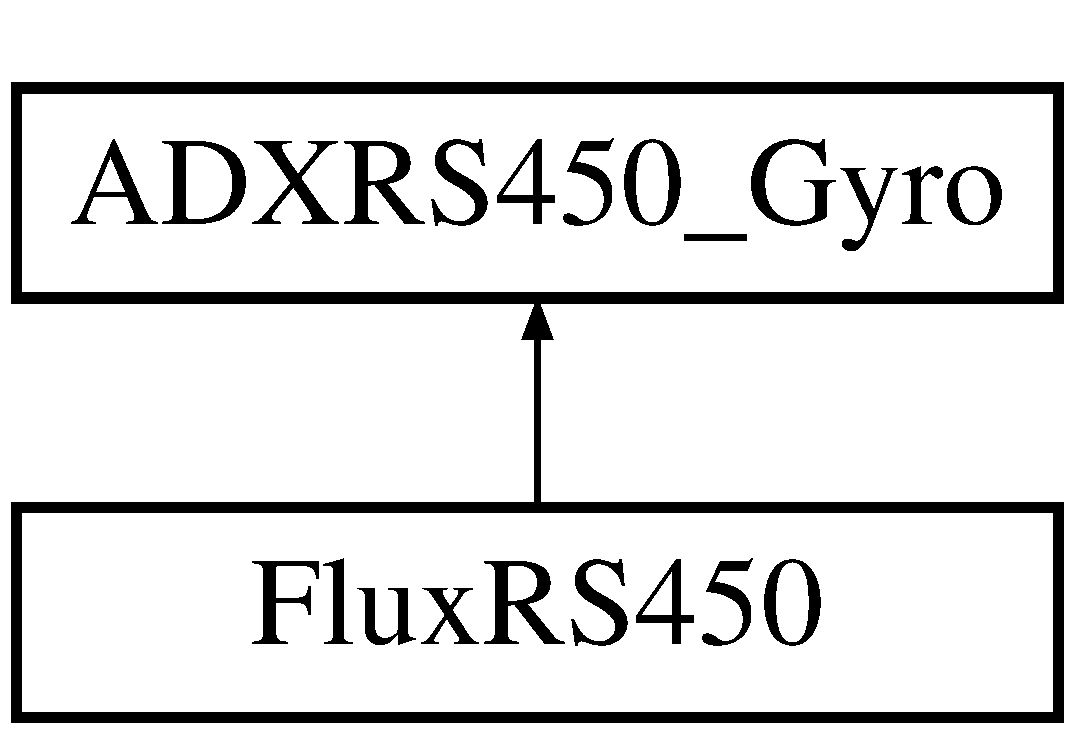
\includegraphics[height=2.000000cm]{classFluxRS450}
\end{center}
\end{figure}
\subsection*{Public Member Functions}
\begin{DoxyCompactItemize}
\item 
void \hyperlink{classFluxRS450_af3c3eaca528a716ab97106fe62936e39}{set\+Target\+Heading} (double \&target\+Heading)
\item 
double \hyperlink{classFluxRS450_ab2642e1b6a64a18b522636de116bca2c}{get\+Target\+Heading} ()
\end{DoxyCompactItemize}
\subsection*{Static Public Member Functions}
\begin{DoxyCompactItemize}
\item 
static \hyperlink{classFluxRS450}{Flux\+R\+S450} \& \hyperlink{classFluxRS450_a14971d76bad4f15cf16ba8642bd79354}{get\+Instance} (S\+P\+I\+::\+Port port\+ID)
\end{DoxyCompactItemize}


\subsection{Detailed Description}
Singleton class for A\+D\+X\+R\+S450 Gyro 

\subsection{Member Function Documentation}
\mbox{\Hypertarget{classFluxRS450_a14971d76bad4f15cf16ba8642bd79354}\label{classFluxRS450_a14971d76bad4f15cf16ba8642bd79354}} 
\index{Flux\+R\+S450@{Flux\+R\+S450}!get\+Instance@{get\+Instance}}
\index{get\+Instance@{get\+Instance}!Flux\+R\+S450@{Flux\+R\+S450}}
\subsubsection{\texorpdfstring{get\+Instance()}{getInstance()}}
{\footnotesize\ttfamily static \hyperlink{classFluxRS450}{Flux\+R\+S450}\& Flux\+R\+S450\+::get\+Instance (\begin{DoxyParamCaption}\item[{S\+P\+I\+::\+Port}]{port\+ID }\end{DoxyParamCaption})\hspace{0.3cm}{\ttfamily [inline]}, {\ttfamily [static]}}

\mbox{\Hypertarget{classFluxRS450_ab2642e1b6a64a18b522636de116bca2c}\label{classFluxRS450_ab2642e1b6a64a18b522636de116bca2c}} 
\index{Flux\+R\+S450@{Flux\+R\+S450}!get\+Target\+Heading@{get\+Target\+Heading}}
\index{get\+Target\+Heading@{get\+Target\+Heading}!Flux\+R\+S450@{Flux\+R\+S450}}
\subsubsection{\texorpdfstring{get\+Target\+Heading()}{getTargetHeading()}}
{\footnotesize\ttfamily double Flux\+R\+S450\+::get\+Target\+Heading (\begin{DoxyParamCaption}{ }\end{DoxyParamCaption})}

\mbox{\Hypertarget{classFluxRS450_af3c3eaca528a716ab97106fe62936e39}\label{classFluxRS450_af3c3eaca528a716ab97106fe62936e39}} 
\index{Flux\+R\+S450@{Flux\+R\+S450}!set\+Target\+Heading@{set\+Target\+Heading}}
\index{set\+Target\+Heading@{set\+Target\+Heading}!Flux\+R\+S450@{Flux\+R\+S450}}
\subsubsection{\texorpdfstring{set\+Target\+Heading()}{setTargetHeading()}}
{\footnotesize\ttfamily void Flux\+R\+S450\+::set\+Target\+Heading (\begin{DoxyParamCaption}\item[{double \&}]{target\+Heading }\end{DoxyParamCaption})}



The documentation for this class was generated from the following files\+:\begin{DoxyCompactItemize}
\item 
src/main/\+Sensors/\hyperlink{FluxRS450_8h}{Flux\+R\+S450.\+h}\item 
src/main/\+Sensors/\hyperlink{FluxRS450_8cpp}{Flux\+R\+S450.\+cpp}\end{DoxyCompactItemize}

\hypertarget{classFluxSubsystem}{}\section{Flux\+Subsystem Class Reference}
\label{classFluxSubsystem}\index{Flux\+Subsystem@{Flux\+Subsystem}}


{\ttfamily \#include $<$Flux\+Subsystem.\+h$>$}

Inheritance diagram for Flux\+Subsystem\+:\begin{figure}[H]
\begin{center}
\leavevmode
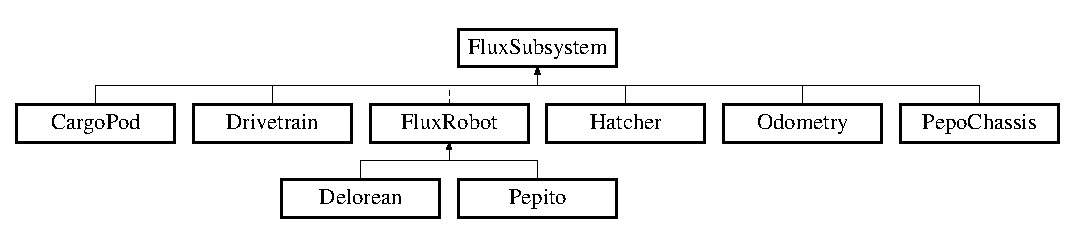
\includegraphics[height=3.000000cm]{classFluxSubsystem}
\end{center}
\end{figure}
\subsection*{Public Member Functions}
\begin{DoxyCompactItemize}
\item 
\hyperlink{classFluxSubsystem_ae1c7aa86576c8b74db9283df11f556d0}{Flux\+Subsystem} (const std\+::string \&name)
\item 
virtual void \hyperlink{classFluxSubsystem_aacd5ddfcadda0866d5e838de09a60d63}{robot\+Init} ()
\item 
virtual void \hyperlink{classFluxSubsystem_ac2b1c08b53251870e945edf7080c1549}{robot\+Update} ()
\item 
virtual void \hyperlink{classFluxSubsystem_aec6d05e4f80c3783684598fb92ad2e55}{teleop\+Init} ()
\item 
virtual void \hyperlink{classFluxSubsystem_a327d76affc60699bfa62563e364e42f5}{teleop\+Update} ()
\item 
virtual void \hyperlink{classFluxSubsystem_a142cb34f612412e26bd0049e037dbe60}{auton\+Init} ()
\item 
virtual void \hyperlink{classFluxSubsystem_aceed900af22503022b8d1278f3693f77}{auton\+Update} ()
\item 
virtual void \hyperlink{classFluxSubsystem_aa0b8fde8aa5094627d15d24e545e1da4}{disabled\+Init} ()
\item 
virtual void \hyperlink{classFluxSubsystem_a5c39cb0f0834cc77a2b8f4f47778da87}{disabled\+Update} ()
\item 
std\+::string \hyperlink{classFluxSubsystem_a661009e388711cd134d519160d1633ac}{get\+Name} () const
\end{DoxyCompactItemize}


\subsection{Detailed Description}
This class is to be used on any subsystem to be implemented on the robot. Functions must be filled when implemented at subsystem writing. Follows Timed\+Robot\textquotesingle{}s structure 

\subsection{Constructor \& Destructor Documentation}
\mbox{\Hypertarget{classFluxSubsystem_ae1c7aa86576c8b74db9283df11f556d0}\label{classFluxSubsystem_ae1c7aa86576c8b74db9283df11f556d0}} 
\index{Flux\+Subsystem@{Flux\+Subsystem}!Flux\+Subsystem@{Flux\+Subsystem}}
\index{Flux\+Subsystem@{Flux\+Subsystem}!Flux\+Subsystem@{Flux\+Subsystem}}
\subsubsection{\texorpdfstring{Flux\+Subsystem()}{FluxSubsystem()}}
{\footnotesize\ttfamily Flux\+Subsystem\+::\+Flux\+Subsystem (\begin{DoxyParamCaption}\item[{const std\+::string \&}]{name }\end{DoxyParamCaption})\hspace{0.3cm}{\ttfamily [explicit]}}



\subsection{Member Function Documentation}
\mbox{\Hypertarget{classFluxSubsystem_a142cb34f612412e26bd0049e037dbe60}\label{classFluxSubsystem_a142cb34f612412e26bd0049e037dbe60}} 
\index{Flux\+Subsystem@{Flux\+Subsystem}!auton\+Init@{auton\+Init}}
\index{auton\+Init@{auton\+Init}!Flux\+Subsystem@{Flux\+Subsystem}}
\subsubsection{\texorpdfstring{auton\+Init()}{autonInit()}}
{\footnotesize\ttfamily void Flux\+Subsystem\+::auton\+Init (\begin{DoxyParamCaption}{ }\end{DoxyParamCaption})\hspace{0.3cm}{\ttfamily [virtual]}}



Reimplemented in \hyperlink{classPepito_ac9a8b75ef48cd95683733af317618ca4}{Pepito}, \hyperlink{classDelorean_ad06990e5c59d5f4d30b48015e744cc49}{Delorean}, \hyperlink{classPepoChassis_a10380f1dad79ff1daa295d0673a1051f}{Pepo\+Chassis}, and \hyperlink{classDrivetrain_a6aec7fa1a9daf1233a59fe0243d3bc8c}{Drivetrain}.

\mbox{\Hypertarget{classFluxSubsystem_aceed900af22503022b8d1278f3693f77}\label{classFluxSubsystem_aceed900af22503022b8d1278f3693f77}} 
\index{Flux\+Subsystem@{Flux\+Subsystem}!auton\+Update@{auton\+Update}}
\index{auton\+Update@{auton\+Update}!Flux\+Subsystem@{Flux\+Subsystem}}
\subsubsection{\texorpdfstring{auton\+Update()}{autonUpdate()}}
{\footnotesize\ttfamily void Flux\+Subsystem\+::auton\+Update (\begin{DoxyParamCaption}{ }\end{DoxyParamCaption})\hspace{0.3cm}{\ttfamily [virtual]}}



Reimplemented in \hyperlink{classPepito_a42cc57495399c63940571b113e7140f8}{Pepito}, \hyperlink{classDelorean_a17c9b875c9c0d3c9b9dadd5838bfedfd}{Delorean}, \hyperlink{classPepoChassis_ab1e73685898517c8fa2f81c5c7a6a56c}{Pepo\+Chassis}, and \hyperlink{classDrivetrain_ab451b48c598fa715ff1a8117ddc6f705}{Drivetrain}.

\mbox{\Hypertarget{classFluxSubsystem_aa0b8fde8aa5094627d15d24e545e1da4}\label{classFluxSubsystem_aa0b8fde8aa5094627d15d24e545e1da4}} 
\index{Flux\+Subsystem@{Flux\+Subsystem}!disabled\+Init@{disabled\+Init}}
\index{disabled\+Init@{disabled\+Init}!Flux\+Subsystem@{Flux\+Subsystem}}
\subsubsection{\texorpdfstring{disabled\+Init()}{disabledInit()}}
{\footnotesize\ttfamily void Flux\+Subsystem\+::disabled\+Init (\begin{DoxyParamCaption}{ }\end{DoxyParamCaption})\hspace{0.3cm}{\ttfamily [virtual]}}



Reimplemented in \hyperlink{classPepito_a04a85eae33c653f9555b6db43d50b210}{Pepito}, \hyperlink{classDelorean_ae054ba79b38b46d20e50becb5d31884c}{Delorean}, \hyperlink{classPepoChassis_af5f6848de51ac4c47cbf2f9f706b1485}{Pepo\+Chassis}, and \hyperlink{classDrivetrain_ac6fe041de609bdb45eac65282fbdf507}{Drivetrain}.

\mbox{\Hypertarget{classFluxSubsystem_a5c39cb0f0834cc77a2b8f4f47778da87}\label{classFluxSubsystem_a5c39cb0f0834cc77a2b8f4f47778da87}} 
\index{Flux\+Subsystem@{Flux\+Subsystem}!disabled\+Update@{disabled\+Update}}
\index{disabled\+Update@{disabled\+Update}!Flux\+Subsystem@{Flux\+Subsystem}}
\subsubsection{\texorpdfstring{disabled\+Update()}{disabledUpdate()}}
{\footnotesize\ttfamily void Flux\+Subsystem\+::disabled\+Update (\begin{DoxyParamCaption}{ }\end{DoxyParamCaption})\hspace{0.3cm}{\ttfamily [virtual]}}



Reimplemented in \hyperlink{classPepito_afc29a2b7ac94a47381ca213dc2993c39}{Pepito}, \hyperlink{classDelorean_acc8f7d93dd894233d16f34316d363983}{Delorean}, \hyperlink{classPepoChassis_a33af04df9c2396d6197f3298172763d9}{Pepo\+Chassis}, and \hyperlink{classDrivetrain_a46aa479a25757868bfda71081ec7baa2}{Drivetrain}.

\mbox{\Hypertarget{classFluxSubsystem_a661009e388711cd134d519160d1633ac}\label{classFluxSubsystem_a661009e388711cd134d519160d1633ac}} 
\index{Flux\+Subsystem@{Flux\+Subsystem}!get\+Name@{get\+Name}}
\index{get\+Name@{get\+Name}!Flux\+Subsystem@{Flux\+Subsystem}}
\subsubsection{\texorpdfstring{get\+Name()}{getName()}}
{\footnotesize\ttfamily std\+::string Flux\+Subsystem\+::get\+Name (\begin{DoxyParamCaption}{ }\end{DoxyParamCaption}) const}

\mbox{\Hypertarget{classFluxSubsystem_aacd5ddfcadda0866d5e838de09a60d63}\label{classFluxSubsystem_aacd5ddfcadda0866d5e838de09a60d63}} 
\index{Flux\+Subsystem@{Flux\+Subsystem}!robot\+Init@{robot\+Init}}
\index{robot\+Init@{robot\+Init}!Flux\+Subsystem@{Flux\+Subsystem}}
\subsubsection{\texorpdfstring{robot\+Init()}{robotInit()}}
{\footnotesize\ttfamily void Flux\+Subsystem\+::robot\+Init (\begin{DoxyParamCaption}{ }\end{DoxyParamCaption})\hspace{0.3cm}{\ttfamily [virtual]}}



Reimplemented in \hyperlink{classPepito_a1eed9bef768f3694d8bdfb4f610b8e3a}{Pepito}, \hyperlink{classDelorean_a591e1b68a21a82c7e1cf4e7dbf5294a2}{Delorean}, \hyperlink{classPepoChassis_a18dd25fff35cf7ccac6b710e329873e6}{Pepo\+Chassis}, and \hyperlink{classDrivetrain_a7e9c10a27b3cc5ad89f2338de39b7c62}{Drivetrain}.

\mbox{\Hypertarget{classFluxSubsystem_ac2b1c08b53251870e945edf7080c1549}\label{classFluxSubsystem_ac2b1c08b53251870e945edf7080c1549}} 
\index{Flux\+Subsystem@{Flux\+Subsystem}!robot\+Update@{robot\+Update}}
\index{robot\+Update@{robot\+Update}!Flux\+Subsystem@{Flux\+Subsystem}}
\subsubsection{\texorpdfstring{robot\+Update()}{robotUpdate()}}
{\footnotesize\ttfamily void Flux\+Subsystem\+::robot\+Update (\begin{DoxyParamCaption}{ }\end{DoxyParamCaption})\hspace{0.3cm}{\ttfamily [virtual]}}



Reimplemented in \hyperlink{classPepito_a0894a64d02550bb35b4e3eefa3ac4934}{Pepito}, \hyperlink{classDelorean_a47b9cfdb59a6f46ee26f45f794e313c1}{Delorean}, \hyperlink{classPepoChassis_acd6fa29da41ac5108af7e3a1f15218aa}{Pepo\+Chassis}, and \hyperlink{classDrivetrain_a2a2b5976426dc0c1f45438fd7a5926e4}{Drivetrain}.

\mbox{\Hypertarget{classFluxSubsystem_aec6d05e4f80c3783684598fb92ad2e55}\label{classFluxSubsystem_aec6d05e4f80c3783684598fb92ad2e55}} 
\index{Flux\+Subsystem@{Flux\+Subsystem}!teleop\+Init@{teleop\+Init}}
\index{teleop\+Init@{teleop\+Init}!Flux\+Subsystem@{Flux\+Subsystem}}
\subsubsection{\texorpdfstring{teleop\+Init()}{teleopInit()}}
{\footnotesize\ttfamily void Flux\+Subsystem\+::teleop\+Init (\begin{DoxyParamCaption}{ }\end{DoxyParamCaption})\hspace{0.3cm}{\ttfamily [virtual]}}



Reimplemented in \hyperlink{classPepito_a5001bee2d7dcc225c87ac36d5eddc452}{Pepito}, \hyperlink{classDelorean_a789c6e4e70f4e2cfdf944d1a1a149509}{Delorean}, \hyperlink{classPepoChassis_a44dbc37a56fe98d7b57af840e8da73b2}{Pepo\+Chassis}, and \hyperlink{classDrivetrain_a12d7edbb3a1b5d4ffa4ecb381c1ab115}{Drivetrain}.

\mbox{\Hypertarget{classFluxSubsystem_a327d76affc60699bfa62563e364e42f5}\label{classFluxSubsystem_a327d76affc60699bfa62563e364e42f5}} 
\index{Flux\+Subsystem@{Flux\+Subsystem}!teleop\+Update@{teleop\+Update}}
\index{teleop\+Update@{teleop\+Update}!Flux\+Subsystem@{Flux\+Subsystem}}
\subsubsection{\texorpdfstring{teleop\+Update()}{teleopUpdate()}}
{\footnotesize\ttfamily void Flux\+Subsystem\+::teleop\+Update (\begin{DoxyParamCaption}{ }\end{DoxyParamCaption})\hspace{0.3cm}{\ttfamily [virtual]}}



Reimplemented in \hyperlink{classPepito_ac19e921b35d2d76cb5b6a2105b26f568}{Pepito}, \hyperlink{classDelorean_a6053dfc106d71fcffa30bac0f5e9b5b8}{Delorean}, \hyperlink{classPepoChassis_af863b7df039af7051b08c051f744e429}{Pepo\+Chassis}, and \hyperlink{classDrivetrain_a3b6bdf96a9388285c7560b2fedfc7ca1}{Drivetrain}.



The documentation for this class was generated from the following files\+:\begin{DoxyCompactItemize}
\item 
src/main/\+Subsystems/\hyperlink{FluxSubsystem_8h}{Flux\+Subsystem.\+h}\item 
src/main/\+Subsystems/\hyperlink{FluxSubsystem_8cpp}{Flux\+Subsystem.\+cpp}\end{DoxyCompactItemize}

\hypertarget{classFluxVictor}{}\section{Flux\+Victor Class Reference}
\label{classFluxVictor}\index{Flux\+Victor@{Flux\+Victor}}


{\ttfamily \#include $<$Flux\+Victor.\+h$>$}

Inheritance diagram for Flux\+Victor\+:\begin{figure}[H]
\begin{center}
\leavevmode
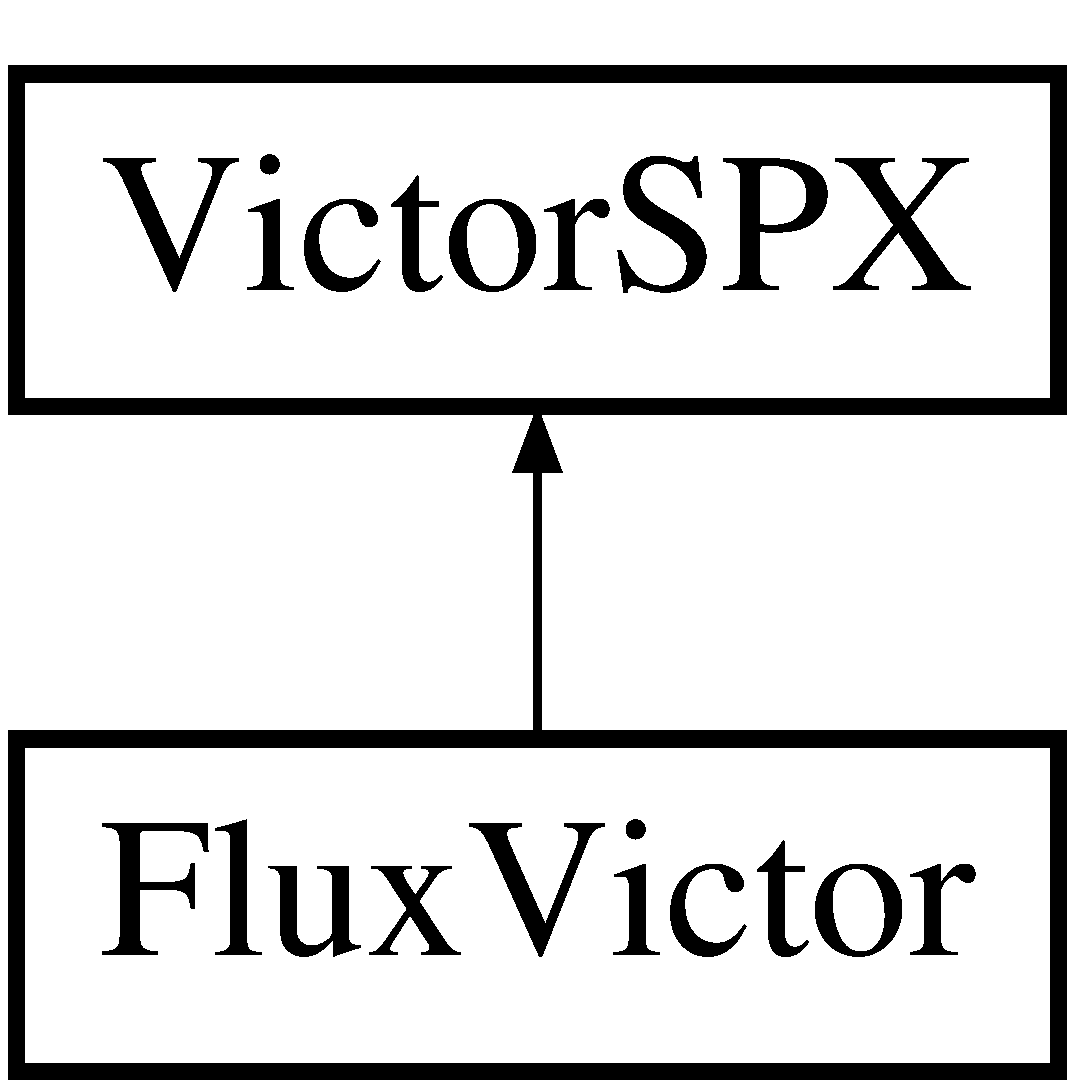
\includegraphics[height=2.000000cm]{classFluxVictor}
\end{center}
\end{figure}
\subsection*{Public Member Functions}
\begin{DoxyCompactItemize}
\item 
\hyperlink{classFluxVictor_aaf6621fe1c9589a10dde59ca9de5a1a0}{Flux\+Victor} (unsigned int port)
\item 
void \hyperlink{classFluxVictor_a84f42f074e9f6d9a3d385f5993e7cc21}{Power} (double input)
\item 
void \hyperlink{classFluxVictor_a6ea20f0e75817153eddf565a33df10c8}{Brake} ()
\end{DoxyCompactItemize}


\subsection{Detailed Description}
Wrapper for Victor\+S\+PX, because syntax sugar. 

\subsection{Constructor \& Destructor Documentation}
\mbox{\Hypertarget{classFluxVictor_aaf6621fe1c9589a10dde59ca9de5a1a0}\label{classFluxVictor_aaf6621fe1c9589a10dde59ca9de5a1a0}} 
\index{Flux\+Victor@{Flux\+Victor}!Flux\+Victor@{Flux\+Victor}}
\index{Flux\+Victor@{Flux\+Victor}!Flux\+Victor@{Flux\+Victor}}
\subsubsection{\texorpdfstring{Flux\+Victor()}{FluxVictor()}}
{\footnotesize\ttfamily Flux\+Victor\+::\+Flux\+Victor (\begin{DoxyParamCaption}\item[{unsigned int}]{port }\end{DoxyParamCaption})}



\subsection{Member Function Documentation}
\mbox{\Hypertarget{classFluxVictor_a6ea20f0e75817153eddf565a33df10c8}\label{classFluxVictor_a6ea20f0e75817153eddf565a33df10c8}} 
\index{Flux\+Victor@{Flux\+Victor}!Brake@{Brake}}
\index{Brake@{Brake}!Flux\+Victor@{Flux\+Victor}}
\subsubsection{\texorpdfstring{Brake()}{Brake()}}
{\footnotesize\ttfamily void Flux\+Victor\+::\+Brake (\begin{DoxyParamCaption}{ }\end{DoxyParamCaption})}

\mbox{\Hypertarget{classFluxVictor_a84f42f074e9f6d9a3d385f5993e7cc21}\label{classFluxVictor_a84f42f074e9f6d9a3d385f5993e7cc21}} 
\index{Flux\+Victor@{Flux\+Victor}!Power@{Power}}
\index{Power@{Power}!Flux\+Victor@{Flux\+Victor}}
\subsubsection{\texorpdfstring{Power()}{Power()}}
{\footnotesize\ttfamily void Flux\+Victor\+::\+Power (\begin{DoxyParamCaption}\item[{double}]{input }\end{DoxyParamCaption})}



The documentation for this class was generated from the following files\+:\begin{DoxyCompactItemize}
\item 
src/main/\+Utilities/\hyperlink{FluxVictor_8h}{Flux\+Victor.\+h}\item 
src/main/\+Utilities/\hyperlink{FluxVictor_8cpp}{Flux\+Victor.\+cpp}\end{DoxyCompactItemize}

\hypertarget{classHatcher}{}\section{Hatcher Class Reference}
\label{classHatcher}\index{Hatcher@{Hatcher}}


{\ttfamily \#include $<$Hatcher.\+h$>$}

Inheritance diagram for Hatcher\+:\begin{figure}[H]
\begin{center}
\leavevmode
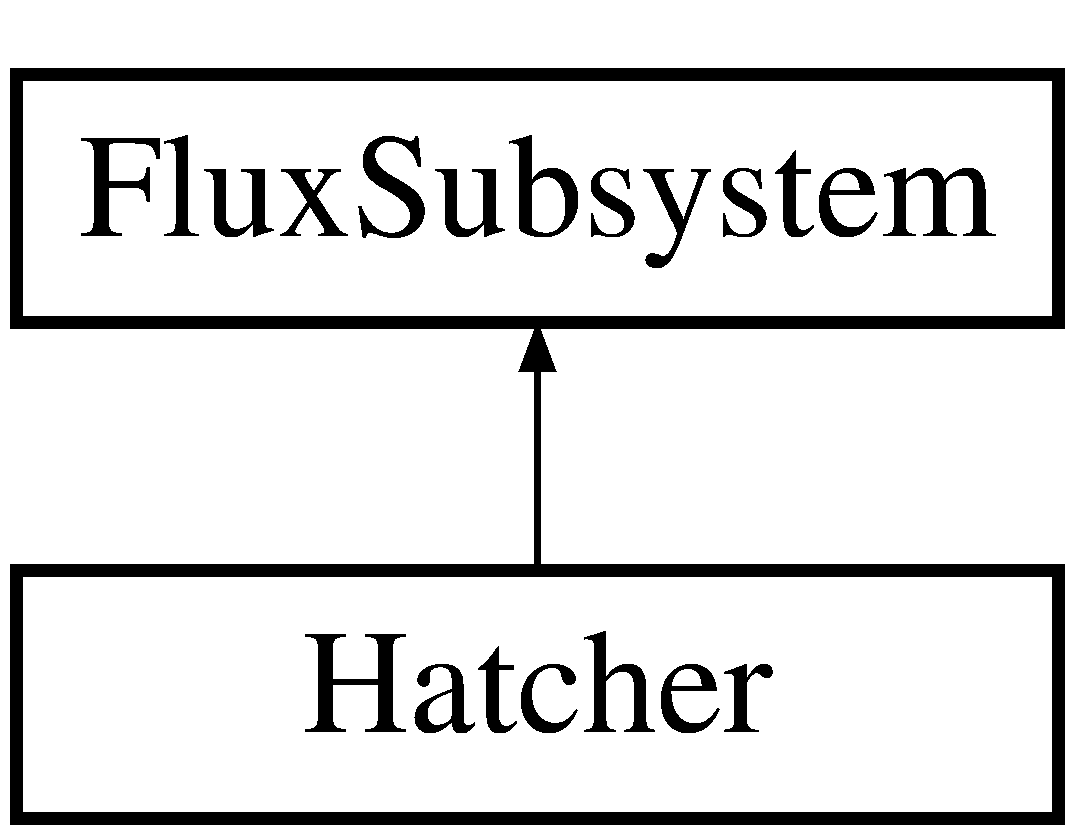
\includegraphics[height=2.000000cm]{classHatcher}
\end{center}
\end{figure}
\subsection*{Public Member Functions}
\begin{DoxyCompactItemize}
\item 
\hyperlink{classHatcher_aa8c7be4eea0af1a3d61b6d445aac487d}{Hatcher} ()
\item 
void \hyperlink{classHatcher_ae917b572274b45c8e695cd8e285a5d70}{robot\+Init} () override
\item 
void \hyperlink{classHatcher_aacf85f8cc9f1c523ef7c4cd91808201e}{robot\+Update} () override
\item 
void \hyperlink{classHatcher_ad51238ccec9093e1fa9c63f8f3aafa12}{teleop\+Init} () override
\item 
void \hyperlink{classHatcher_a91517b2f54f6c8fc0f27506963a71d20}{teleop\+Update} () override
\item 
void \hyperlink{classHatcher_a2e61639f734ec3a5627b655695bbadf1}{disabled\+Init} () override
\item 
void \hyperlink{classHatcher_ab6bb222ab940507490f2009f3113bc41}{disabled\+Update} () override
\item 
void \hyperlink{classHatcher_ac44bea31eb17578106c48914450a1be1}{auton\+Init} () override
\item 
void \hyperlink{classHatcher_a5e21dc019a7f05b4bbbf39545a920f5a}{auton\+Update} () override
\end{DoxyCompactItemize}


\subsection{Constructor \& Destructor Documentation}
\mbox{\Hypertarget{classHatcher_aa8c7be4eea0af1a3d61b6d445aac487d}\label{classHatcher_aa8c7be4eea0af1a3d61b6d445aac487d}} 
\index{Hatcher@{Hatcher}!Hatcher@{Hatcher}}
\index{Hatcher@{Hatcher}!Hatcher@{Hatcher}}
\subsubsection{\texorpdfstring{Hatcher()}{Hatcher()}}
{\footnotesize\ttfamily Hatcher\+::\+Hatcher (\begin{DoxyParamCaption}{ }\end{DoxyParamCaption})}



\subsection{Member Function Documentation}
\mbox{\Hypertarget{classHatcher_ac44bea31eb17578106c48914450a1be1}\label{classHatcher_ac44bea31eb17578106c48914450a1be1}} 
\index{Hatcher@{Hatcher}!auton\+Init@{auton\+Init}}
\index{auton\+Init@{auton\+Init}!Hatcher@{Hatcher}}
\subsubsection{\texorpdfstring{auton\+Init()}{autonInit()}}
{\footnotesize\ttfamily void Hatcher\+::auton\+Init (\begin{DoxyParamCaption}{ }\end{DoxyParamCaption})\hspace{0.3cm}{\ttfamily [override]}, {\ttfamily [virtual]}}



Reimplemented from \hyperlink{classFluxSubsystem_a142cb34f612412e26bd0049e037dbe60}{Flux\+Subsystem}.

\mbox{\Hypertarget{classHatcher_a5e21dc019a7f05b4bbbf39545a920f5a}\label{classHatcher_a5e21dc019a7f05b4bbbf39545a920f5a}} 
\index{Hatcher@{Hatcher}!auton\+Update@{auton\+Update}}
\index{auton\+Update@{auton\+Update}!Hatcher@{Hatcher}}
\subsubsection{\texorpdfstring{auton\+Update()}{autonUpdate()}}
{\footnotesize\ttfamily void Hatcher\+::auton\+Update (\begin{DoxyParamCaption}{ }\end{DoxyParamCaption})\hspace{0.3cm}{\ttfamily [override]}, {\ttfamily [virtual]}}



Reimplemented from \hyperlink{classFluxSubsystem_aceed900af22503022b8d1278f3693f77}{Flux\+Subsystem}.

\mbox{\Hypertarget{classHatcher_a2e61639f734ec3a5627b655695bbadf1}\label{classHatcher_a2e61639f734ec3a5627b655695bbadf1}} 
\index{Hatcher@{Hatcher}!disabled\+Init@{disabled\+Init}}
\index{disabled\+Init@{disabled\+Init}!Hatcher@{Hatcher}}
\subsubsection{\texorpdfstring{disabled\+Init()}{disabledInit()}}
{\footnotesize\ttfamily void Hatcher\+::disabled\+Init (\begin{DoxyParamCaption}{ }\end{DoxyParamCaption})\hspace{0.3cm}{\ttfamily [override]}, {\ttfamily [virtual]}}



Reimplemented from \hyperlink{classFluxSubsystem_aa0b8fde8aa5094627d15d24e545e1da4}{Flux\+Subsystem}.

\mbox{\Hypertarget{classHatcher_ab6bb222ab940507490f2009f3113bc41}\label{classHatcher_ab6bb222ab940507490f2009f3113bc41}} 
\index{Hatcher@{Hatcher}!disabled\+Update@{disabled\+Update}}
\index{disabled\+Update@{disabled\+Update}!Hatcher@{Hatcher}}
\subsubsection{\texorpdfstring{disabled\+Update()}{disabledUpdate()}}
{\footnotesize\ttfamily void Hatcher\+::disabled\+Update (\begin{DoxyParamCaption}{ }\end{DoxyParamCaption})\hspace{0.3cm}{\ttfamily [override]}, {\ttfamily [virtual]}}



Reimplemented from \hyperlink{classFluxSubsystem_a5c39cb0f0834cc77a2b8f4f47778da87}{Flux\+Subsystem}.

\mbox{\Hypertarget{classHatcher_ae917b572274b45c8e695cd8e285a5d70}\label{classHatcher_ae917b572274b45c8e695cd8e285a5d70}} 
\index{Hatcher@{Hatcher}!robot\+Init@{robot\+Init}}
\index{robot\+Init@{robot\+Init}!Hatcher@{Hatcher}}
\subsubsection{\texorpdfstring{robot\+Init()}{robotInit()}}
{\footnotesize\ttfamily void Hatcher\+::robot\+Init (\begin{DoxyParamCaption}{ }\end{DoxyParamCaption})\hspace{0.3cm}{\ttfamily [override]}, {\ttfamily [virtual]}}



Reimplemented from \hyperlink{classFluxSubsystem_aacd5ddfcadda0866d5e838de09a60d63}{Flux\+Subsystem}.

\mbox{\Hypertarget{classHatcher_aacf85f8cc9f1c523ef7c4cd91808201e}\label{classHatcher_aacf85f8cc9f1c523ef7c4cd91808201e}} 
\index{Hatcher@{Hatcher}!robot\+Update@{robot\+Update}}
\index{robot\+Update@{robot\+Update}!Hatcher@{Hatcher}}
\subsubsection{\texorpdfstring{robot\+Update()}{robotUpdate()}}
{\footnotesize\ttfamily void Hatcher\+::robot\+Update (\begin{DoxyParamCaption}{ }\end{DoxyParamCaption})\hspace{0.3cm}{\ttfamily [override]}, {\ttfamily [virtual]}}



Reimplemented from \hyperlink{classFluxSubsystem_ac2b1c08b53251870e945edf7080c1549}{Flux\+Subsystem}.

\mbox{\Hypertarget{classHatcher_ad51238ccec9093e1fa9c63f8f3aafa12}\label{classHatcher_ad51238ccec9093e1fa9c63f8f3aafa12}} 
\index{Hatcher@{Hatcher}!teleop\+Init@{teleop\+Init}}
\index{teleop\+Init@{teleop\+Init}!Hatcher@{Hatcher}}
\subsubsection{\texorpdfstring{teleop\+Init()}{teleopInit()}}
{\footnotesize\ttfamily void Hatcher\+::teleop\+Init (\begin{DoxyParamCaption}{ }\end{DoxyParamCaption})\hspace{0.3cm}{\ttfamily [override]}, {\ttfamily [virtual]}}



Reimplemented from \hyperlink{classFluxSubsystem_aec6d05e4f80c3783684598fb92ad2e55}{Flux\+Subsystem}.

\mbox{\Hypertarget{classHatcher_a91517b2f54f6c8fc0f27506963a71d20}\label{classHatcher_a91517b2f54f6c8fc0f27506963a71d20}} 
\index{Hatcher@{Hatcher}!teleop\+Update@{teleop\+Update}}
\index{teleop\+Update@{teleop\+Update}!Hatcher@{Hatcher}}
\subsubsection{\texorpdfstring{teleop\+Update()}{teleopUpdate()}}
{\footnotesize\ttfamily void Hatcher\+::teleop\+Update (\begin{DoxyParamCaption}{ }\end{DoxyParamCaption})\hspace{0.3cm}{\ttfamily [override]}, {\ttfamily [virtual]}}



Reimplemented from \hyperlink{classFluxSubsystem_a327d76affc60699bfa62563e364e42f5}{Flux\+Subsystem}.



The documentation for this class was generated from the following files\+:\begin{DoxyCompactItemize}
\item 
src/main/2019/\+Mechs/\hyperlink{Hatcher_8h}{Hatcher.\+h}\item 
src/main/2019/\+Mechs/\hyperlink{Hatcher_8cpp}{Hatcher.\+cpp}\end{DoxyCompactItemize}

\hypertarget{classOdometry}{}\section{Odometry Class Reference}
\label{classOdometry}\index{Odometry@{Odometry}}


{\ttfamily \#include $<$Odometry.\+h$>$}

Inheritance diagram for Odometry\+:\begin{figure}[H]
\begin{center}
\leavevmode
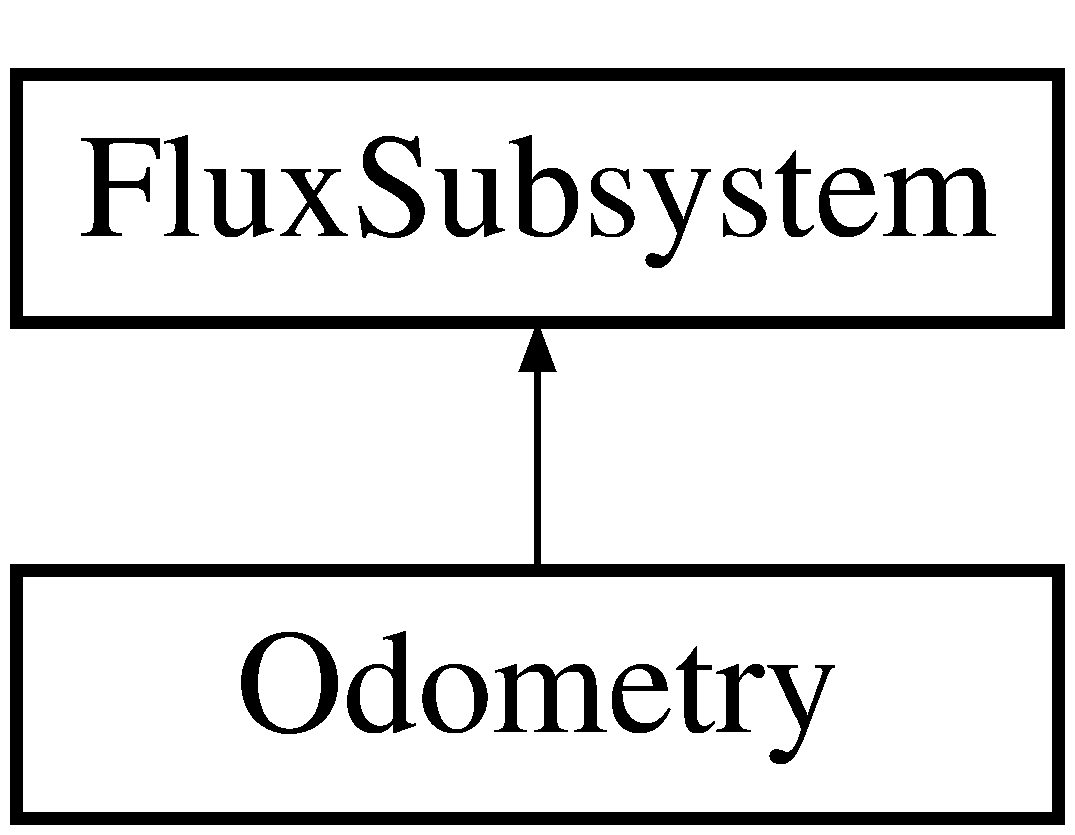
\includegraphics[height=2.000000cm]{classOdometry}
\end{center}
\end{figure}
\subsection*{Public Member Functions}
\begin{DoxyCompactItemize}
\item 
\hyperlink{classOdometry_a54b672ac09bd117fa04773f131492c35}{Odometry} ()
\item 
void \hyperlink{classOdometry_a84379c5878ad6dd502297e6f956298f9}{robot\+Init} () override
\item 
void \hyperlink{classOdometry_a4c82fa784546795d6b0bf32c1b919202}{robot\+Update} () override
\item 
void \hyperlink{classOdometry_adea396ff746c1f3ad73ea79d19a75356}{teleop\+Init} () override
\item 
void \hyperlink{classOdometry_ae42a153c786b5c805b073509394951f9}{teleop\+Update} () override
\item 
void \hyperlink{classOdometry_a0ec037096f65e779248e6a99615f37ed}{auton\+Init} () override
\item 
void \hyperlink{classOdometry_a5a19f4d904e5364ca75a91f97a8777a6}{auton\+Update} () override
\item 
void \hyperlink{classOdometry_a0df3b0180a8fa5a01a9e441de112140e}{disabled\+Init} () override
\item 
void \hyperlink{classOdometry_aef83c6c62c8e992b20759aec705c2ee8}{disabled\+Update} () override
\end{DoxyCompactItemize}


\subsection{Constructor \& Destructor Documentation}
\mbox{\Hypertarget{classOdometry_a54b672ac09bd117fa04773f131492c35}\label{classOdometry_a54b672ac09bd117fa04773f131492c35}} 
\index{Odometry@{Odometry}!Odometry@{Odometry}}
\index{Odometry@{Odometry}!Odometry@{Odometry}}
\subsubsection{\texorpdfstring{Odometry()}{Odometry()}}
{\footnotesize\ttfamily Odometry\+::\+Odometry (\begin{DoxyParamCaption}{ }\end{DoxyParamCaption})}



\subsection{Member Function Documentation}
\mbox{\Hypertarget{classOdometry_a0ec037096f65e779248e6a99615f37ed}\label{classOdometry_a0ec037096f65e779248e6a99615f37ed}} 
\index{Odometry@{Odometry}!auton\+Init@{auton\+Init}}
\index{auton\+Init@{auton\+Init}!Odometry@{Odometry}}
\subsubsection{\texorpdfstring{auton\+Init()}{autonInit()}}
{\footnotesize\ttfamily void Odometry\+::auton\+Init (\begin{DoxyParamCaption}{ }\end{DoxyParamCaption})\hspace{0.3cm}{\ttfamily [override]}, {\ttfamily [virtual]}}



Reimplemented from \hyperlink{classFluxSubsystem_a142cb34f612412e26bd0049e037dbe60}{Flux\+Subsystem}.

\mbox{\Hypertarget{classOdometry_a5a19f4d904e5364ca75a91f97a8777a6}\label{classOdometry_a5a19f4d904e5364ca75a91f97a8777a6}} 
\index{Odometry@{Odometry}!auton\+Update@{auton\+Update}}
\index{auton\+Update@{auton\+Update}!Odometry@{Odometry}}
\subsubsection{\texorpdfstring{auton\+Update()}{autonUpdate()}}
{\footnotesize\ttfamily void Odometry\+::auton\+Update (\begin{DoxyParamCaption}{ }\end{DoxyParamCaption})\hspace{0.3cm}{\ttfamily [override]}, {\ttfamily [virtual]}}



Reimplemented from \hyperlink{classFluxSubsystem_aceed900af22503022b8d1278f3693f77}{Flux\+Subsystem}.

\mbox{\Hypertarget{classOdometry_a0df3b0180a8fa5a01a9e441de112140e}\label{classOdometry_a0df3b0180a8fa5a01a9e441de112140e}} 
\index{Odometry@{Odometry}!disabled\+Init@{disabled\+Init}}
\index{disabled\+Init@{disabled\+Init}!Odometry@{Odometry}}
\subsubsection{\texorpdfstring{disabled\+Init()}{disabledInit()}}
{\footnotesize\ttfamily void Odometry\+::disabled\+Init (\begin{DoxyParamCaption}{ }\end{DoxyParamCaption})\hspace{0.3cm}{\ttfamily [override]}, {\ttfamily [virtual]}}



Reimplemented from \hyperlink{classFluxSubsystem_aa0b8fde8aa5094627d15d24e545e1da4}{Flux\+Subsystem}.

\mbox{\Hypertarget{classOdometry_aef83c6c62c8e992b20759aec705c2ee8}\label{classOdometry_aef83c6c62c8e992b20759aec705c2ee8}} 
\index{Odometry@{Odometry}!disabled\+Update@{disabled\+Update}}
\index{disabled\+Update@{disabled\+Update}!Odometry@{Odometry}}
\subsubsection{\texorpdfstring{disabled\+Update()}{disabledUpdate()}}
{\footnotesize\ttfamily void Odometry\+::disabled\+Update (\begin{DoxyParamCaption}{ }\end{DoxyParamCaption})\hspace{0.3cm}{\ttfamily [override]}, {\ttfamily [virtual]}}



Reimplemented from \hyperlink{classFluxSubsystem_a5c39cb0f0834cc77a2b8f4f47778da87}{Flux\+Subsystem}.

\mbox{\Hypertarget{classOdometry_a84379c5878ad6dd502297e6f956298f9}\label{classOdometry_a84379c5878ad6dd502297e6f956298f9}} 
\index{Odometry@{Odometry}!robot\+Init@{robot\+Init}}
\index{robot\+Init@{robot\+Init}!Odometry@{Odometry}}
\subsubsection{\texorpdfstring{robot\+Init()}{robotInit()}}
{\footnotesize\ttfamily void Odometry\+::robot\+Init (\begin{DoxyParamCaption}{ }\end{DoxyParamCaption})\hspace{0.3cm}{\ttfamily [override]}, {\ttfamily [virtual]}}



Reimplemented from \hyperlink{classFluxSubsystem_aacd5ddfcadda0866d5e838de09a60d63}{Flux\+Subsystem}.

\mbox{\Hypertarget{classOdometry_a4c82fa784546795d6b0bf32c1b919202}\label{classOdometry_a4c82fa784546795d6b0bf32c1b919202}} 
\index{Odometry@{Odometry}!robot\+Update@{robot\+Update}}
\index{robot\+Update@{robot\+Update}!Odometry@{Odometry}}
\subsubsection{\texorpdfstring{robot\+Update()}{robotUpdate()}}
{\footnotesize\ttfamily void Odometry\+::robot\+Update (\begin{DoxyParamCaption}{ }\end{DoxyParamCaption})\hspace{0.3cm}{\ttfamily [override]}, {\ttfamily [virtual]}}



Reimplemented from \hyperlink{classFluxSubsystem_ac2b1c08b53251870e945edf7080c1549}{Flux\+Subsystem}.

\mbox{\Hypertarget{classOdometry_adea396ff746c1f3ad73ea79d19a75356}\label{classOdometry_adea396ff746c1f3ad73ea79d19a75356}} 
\index{Odometry@{Odometry}!teleop\+Init@{teleop\+Init}}
\index{teleop\+Init@{teleop\+Init}!Odometry@{Odometry}}
\subsubsection{\texorpdfstring{teleop\+Init()}{teleopInit()}}
{\footnotesize\ttfamily void Odometry\+::teleop\+Init (\begin{DoxyParamCaption}{ }\end{DoxyParamCaption})\hspace{0.3cm}{\ttfamily [override]}, {\ttfamily [virtual]}}



Reimplemented from \hyperlink{classFluxSubsystem_aec6d05e4f80c3783684598fb92ad2e55}{Flux\+Subsystem}.

\mbox{\Hypertarget{classOdometry_ae42a153c786b5c805b073509394951f9}\label{classOdometry_ae42a153c786b5c805b073509394951f9}} 
\index{Odometry@{Odometry}!teleop\+Update@{teleop\+Update}}
\index{teleop\+Update@{teleop\+Update}!Odometry@{Odometry}}
\subsubsection{\texorpdfstring{teleop\+Update()}{teleopUpdate()}}
{\footnotesize\ttfamily void Odometry\+::teleop\+Update (\begin{DoxyParamCaption}{ }\end{DoxyParamCaption})\hspace{0.3cm}{\ttfamily [override]}, {\ttfamily [virtual]}}



Reimplemented from \hyperlink{classFluxSubsystem_a327d76affc60699bfa62563e364e42f5}{Flux\+Subsystem}.



The documentation for this class was generated from the following file\+:\begin{DoxyCompactItemize}
\item 
src/main/\+Sensors/\hyperlink{Odometry_8h}{Odometry.\+h}\end{DoxyCompactItemize}

\hypertarget{classPepito}{}\section{Pepito Class Reference}
\label{classPepito}\index{Pepito@{Pepito}}


{\ttfamily \#include $<$Pepito.\+h$>$}

Inheritance diagram for Pepito\+:\begin{figure}[H]
\begin{center}
\leavevmode
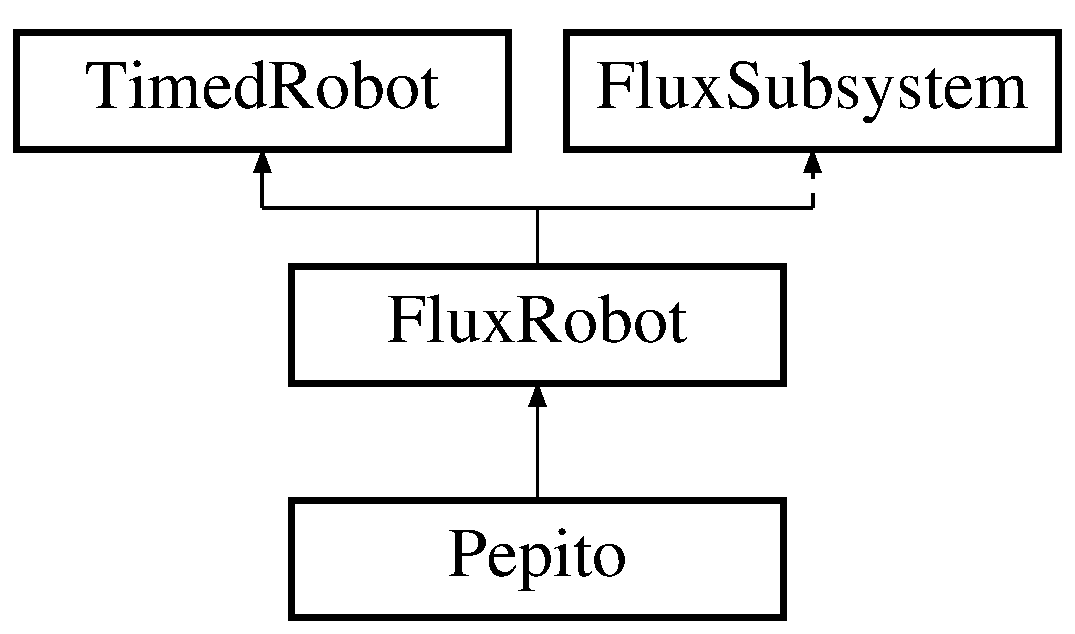
\includegraphics[height=3.000000cm]{classPepito}
\end{center}
\end{figure}
\subsection*{Public Member Functions}
\begin{DoxyCompactItemize}
\item 
\hyperlink{classPepito_a5cfed0e7fc2f459c9dd983e44f46ae53}{Pepito} ()
\item 
void \hyperlink{classPepito_a1368f048f197d9b0e3a7e710dd4809fc}{add\+Properties} () override
\item 
void \hyperlink{classPepito_a420a3322a1fa658e9e40f277e7cc1c03}{init\+Subsystems} () override
\item 
void \hyperlink{classPepito_a1eed9bef768f3694d8bdfb4f610b8e3a}{robot\+Init} () override
\item 
void \hyperlink{classPepito_a0894a64d02550bb35b4e3eefa3ac4934}{robot\+Update} () override
\item 
void \hyperlink{classPepito_a5001bee2d7dcc225c87ac36d5eddc452}{teleop\+Init} () override
\item 
void \hyperlink{classPepito_ac19e921b35d2d76cb5b6a2105b26f568}{teleop\+Update} () override
\item 
void \hyperlink{classPepito_ac9a8b75ef48cd95683733af317618ca4}{auton\+Init} () override
\item 
void \hyperlink{classPepito_a42cc57495399c63940571b113e7140f8}{auton\+Update} () override
\item 
void \hyperlink{classPepito_a04a85eae33c653f9555b6db43d50b210}{disabled\+Init} () override
\item 
void \hyperlink{classPepito_afc29a2b7ac94a47381ca213dc2993c39}{disabled\+Update} () override
\end{DoxyCompactItemize}
\subsection*{Additional Inherited Members}


\subsection{Constructor \& Destructor Documentation}
\mbox{\Hypertarget{classPepito_a5cfed0e7fc2f459c9dd983e44f46ae53}\label{classPepito_a5cfed0e7fc2f459c9dd983e44f46ae53}} 
\index{Pepito@{Pepito}!Pepito@{Pepito}}
\index{Pepito@{Pepito}!Pepito@{Pepito}}
\subsubsection{\texorpdfstring{Pepito()}{Pepito()}}
{\footnotesize\ttfamily Pepito\+::\+Pepito (\begin{DoxyParamCaption}{ }\end{DoxyParamCaption})}



\subsection{Member Function Documentation}
\mbox{\Hypertarget{classPepito_a1368f048f197d9b0e3a7e710dd4809fc}\label{classPepito_a1368f048f197d9b0e3a7e710dd4809fc}} 
\index{Pepito@{Pepito}!add\+Properties@{add\+Properties}}
\index{add\+Properties@{add\+Properties}!Pepito@{Pepito}}
\subsubsection{\texorpdfstring{add\+Properties()}{addProperties()}}
{\footnotesize\ttfamily void Pepito\+::add\+Properties (\begin{DoxyParamCaption}{ }\end{DoxyParamCaption})\hspace{0.3cm}{\ttfamily [override]}, {\ttfamily [virtual]}}



Implements \hyperlink{classFluxRobot_a6f7940d8f82e80a6e405bad20ec9a5a5}{Flux\+Robot}.

\mbox{\Hypertarget{classPepito_ac9a8b75ef48cd95683733af317618ca4}\label{classPepito_ac9a8b75ef48cd95683733af317618ca4}} 
\index{Pepito@{Pepito}!auton\+Init@{auton\+Init}}
\index{auton\+Init@{auton\+Init}!Pepito@{Pepito}}
\subsubsection{\texorpdfstring{auton\+Init()}{autonInit()}}
{\footnotesize\ttfamily void Pepito\+::auton\+Init (\begin{DoxyParamCaption}{ }\end{DoxyParamCaption})\hspace{0.3cm}{\ttfamily [override]}, {\ttfamily [virtual]}}



Reimplemented from \hyperlink{classFluxSubsystem_a142cb34f612412e26bd0049e037dbe60}{Flux\+Subsystem}.

\mbox{\Hypertarget{classPepito_a42cc57495399c63940571b113e7140f8}\label{classPepito_a42cc57495399c63940571b113e7140f8}} 
\index{Pepito@{Pepito}!auton\+Update@{auton\+Update}}
\index{auton\+Update@{auton\+Update}!Pepito@{Pepito}}
\subsubsection{\texorpdfstring{auton\+Update()}{autonUpdate()}}
{\footnotesize\ttfamily void Pepito\+::auton\+Update (\begin{DoxyParamCaption}{ }\end{DoxyParamCaption})\hspace{0.3cm}{\ttfamily [override]}, {\ttfamily [virtual]}}



Reimplemented from \hyperlink{classFluxSubsystem_aceed900af22503022b8d1278f3693f77}{Flux\+Subsystem}.

\mbox{\Hypertarget{classPepito_a04a85eae33c653f9555b6db43d50b210}\label{classPepito_a04a85eae33c653f9555b6db43d50b210}} 
\index{Pepito@{Pepito}!disabled\+Init@{disabled\+Init}}
\index{disabled\+Init@{disabled\+Init}!Pepito@{Pepito}}
\subsubsection{\texorpdfstring{disabled\+Init()}{disabledInit()}}
{\footnotesize\ttfamily void Pepito\+::disabled\+Init (\begin{DoxyParamCaption}{ }\end{DoxyParamCaption})\hspace{0.3cm}{\ttfamily [override]}, {\ttfamily [virtual]}}



Reimplemented from \hyperlink{classFluxSubsystem_aa0b8fde8aa5094627d15d24e545e1da4}{Flux\+Subsystem}.

\mbox{\Hypertarget{classPepito_afc29a2b7ac94a47381ca213dc2993c39}\label{classPepito_afc29a2b7ac94a47381ca213dc2993c39}} 
\index{Pepito@{Pepito}!disabled\+Update@{disabled\+Update}}
\index{disabled\+Update@{disabled\+Update}!Pepito@{Pepito}}
\subsubsection{\texorpdfstring{disabled\+Update()}{disabledUpdate()}}
{\footnotesize\ttfamily void Pepito\+::disabled\+Update (\begin{DoxyParamCaption}{ }\end{DoxyParamCaption})\hspace{0.3cm}{\ttfamily [override]}, {\ttfamily [virtual]}}



Reimplemented from \hyperlink{classFluxSubsystem_a5c39cb0f0834cc77a2b8f4f47778da87}{Flux\+Subsystem}.

\mbox{\Hypertarget{classPepito_a420a3322a1fa658e9e40f277e7cc1c03}\label{classPepito_a420a3322a1fa658e9e40f277e7cc1c03}} 
\index{Pepito@{Pepito}!init\+Subsystems@{init\+Subsystems}}
\index{init\+Subsystems@{init\+Subsystems}!Pepito@{Pepito}}
\subsubsection{\texorpdfstring{init\+Subsystems()}{initSubsystems()}}
{\footnotesize\ttfamily void Pepito\+::init\+Subsystems (\begin{DoxyParamCaption}{ }\end{DoxyParamCaption})\hspace{0.3cm}{\ttfamily [override]}, {\ttfamily [virtual]}}

Add subsystems here 

Implements \hyperlink{classFluxRobot_aa5fcf98b4dfd539b1b49772381578dc8}{Flux\+Robot}.

\mbox{\Hypertarget{classPepito_a1eed9bef768f3694d8bdfb4f610b8e3a}\label{classPepito_a1eed9bef768f3694d8bdfb4f610b8e3a}} 
\index{Pepito@{Pepito}!robot\+Init@{robot\+Init}}
\index{robot\+Init@{robot\+Init}!Pepito@{Pepito}}
\subsubsection{\texorpdfstring{robot\+Init()}{robotInit()}}
{\footnotesize\ttfamily void Pepito\+::robot\+Init (\begin{DoxyParamCaption}{ }\end{DoxyParamCaption})\hspace{0.3cm}{\ttfamily [override]}, {\ttfamily [virtual]}}



Reimplemented from \hyperlink{classFluxSubsystem_aacd5ddfcadda0866d5e838de09a60d63}{Flux\+Subsystem}.

\mbox{\Hypertarget{classPepito_a0894a64d02550bb35b4e3eefa3ac4934}\label{classPepito_a0894a64d02550bb35b4e3eefa3ac4934}} 
\index{Pepito@{Pepito}!robot\+Update@{robot\+Update}}
\index{robot\+Update@{robot\+Update}!Pepito@{Pepito}}
\subsubsection{\texorpdfstring{robot\+Update()}{robotUpdate()}}
{\footnotesize\ttfamily void Pepito\+::robot\+Update (\begin{DoxyParamCaption}{ }\end{DoxyParamCaption})\hspace{0.3cm}{\ttfamily [override]}, {\ttfamily [virtual]}}



Reimplemented from \hyperlink{classFluxSubsystem_ac2b1c08b53251870e945edf7080c1549}{Flux\+Subsystem}.

\mbox{\Hypertarget{classPepito_a5001bee2d7dcc225c87ac36d5eddc452}\label{classPepito_a5001bee2d7dcc225c87ac36d5eddc452}} 
\index{Pepito@{Pepito}!teleop\+Init@{teleop\+Init}}
\index{teleop\+Init@{teleop\+Init}!Pepito@{Pepito}}
\subsubsection{\texorpdfstring{teleop\+Init()}{teleopInit()}}
{\footnotesize\ttfamily void Pepito\+::teleop\+Init (\begin{DoxyParamCaption}{ }\end{DoxyParamCaption})\hspace{0.3cm}{\ttfamily [override]}, {\ttfamily [virtual]}}



Reimplemented from \hyperlink{classFluxSubsystem_aec6d05e4f80c3783684598fb92ad2e55}{Flux\+Subsystem}.

\mbox{\Hypertarget{classPepito_ac19e921b35d2d76cb5b6a2105b26f568}\label{classPepito_ac19e921b35d2d76cb5b6a2105b26f568}} 
\index{Pepito@{Pepito}!teleop\+Update@{teleop\+Update}}
\index{teleop\+Update@{teleop\+Update}!Pepito@{Pepito}}
\subsubsection{\texorpdfstring{teleop\+Update()}{teleopUpdate()}}
{\footnotesize\ttfamily void Pepito\+::teleop\+Update (\begin{DoxyParamCaption}{ }\end{DoxyParamCaption})\hspace{0.3cm}{\ttfamily [override]}, {\ttfamily [virtual]}}



Reimplemented from \hyperlink{classFluxSubsystem_a327d76affc60699bfa62563e364e42f5}{Flux\+Subsystem}.



The documentation for this class was generated from the following files\+:\begin{DoxyCompactItemize}
\item 
src/main/2019/\+Pepito/\hyperlink{Pepito_8h}{Pepito.\+h}\item 
src/main/2019/\+Pepito/\hyperlink{Pepito_8cpp}{Pepito.\+cpp}\end{DoxyCompactItemize}

\hypertarget{classPepoChassis}{}\section{Pepo\+Chassis Class Reference}
\label{classPepoChassis}\index{Pepo\+Chassis@{Pepo\+Chassis}}


{\ttfamily \#include $<$Pepochassis.\+h$>$}

Inheritance diagram for Pepo\+Chassis\+:\begin{figure}[H]
\begin{center}
\leavevmode
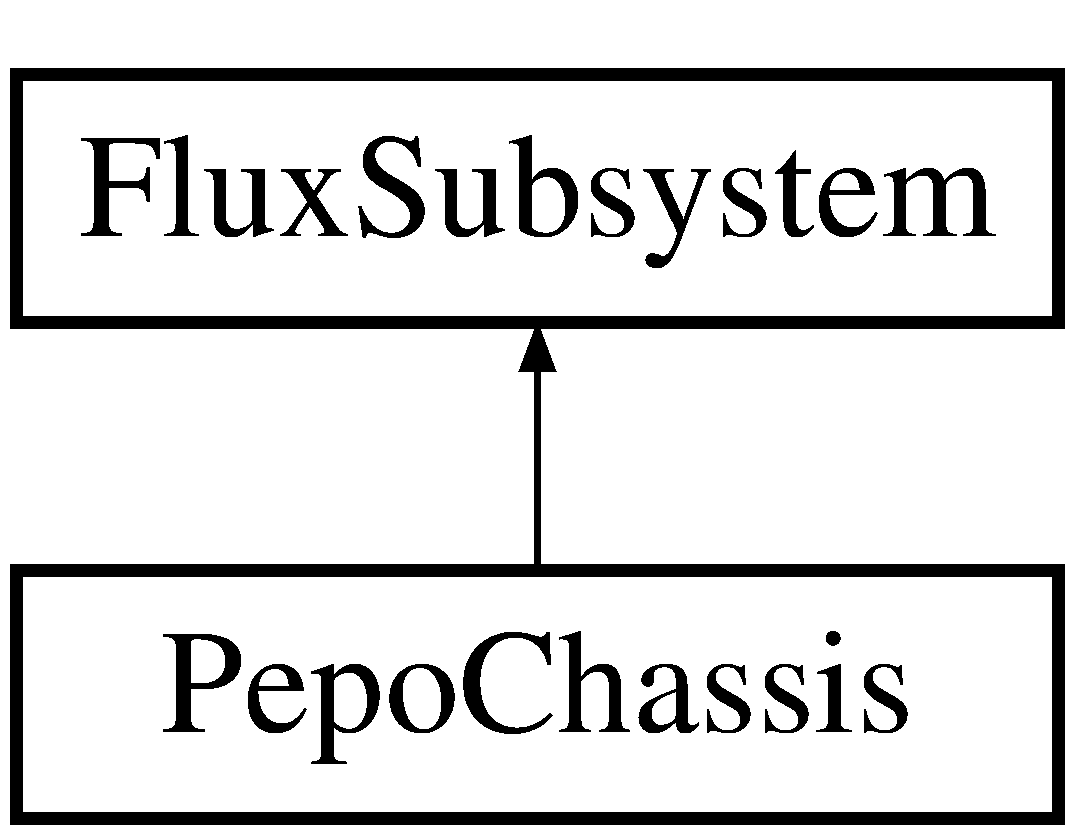
\includegraphics[height=2.000000cm]{classPepoChassis}
\end{center}
\end{figure}
\subsection*{Public Member Functions}
\begin{DoxyCompactItemize}
\item 
\hyperlink{classPepoChassis_a7671239e4338a851b31322b743e1d648}{Pepo\+Chassis} (Victor\+S\+PX \&left\+Victor, Victor\+S\+PX \&right\+Victor, double ramp)
\item 
void \hyperlink{classPepoChassis_a18dd25fff35cf7ccac6b710e329873e6}{robot\+Init} () override
\item 
void \hyperlink{classPepoChassis_acd6fa29da41ac5108af7e3a1f15218aa}{robot\+Update} () override
\item 
void \hyperlink{classPepoChassis_a44dbc37a56fe98d7b57af840e8da73b2}{teleop\+Init} () override
\item 
void \hyperlink{classPepoChassis_af863b7df039af7051b08c051f744e429}{teleop\+Update} () override
\item 
void \hyperlink{classPepoChassis_a10380f1dad79ff1daa295d0673a1051f}{auton\+Init} () override
\item 
void \hyperlink{classPepoChassis_ab1e73685898517c8fa2f81c5c7a6a56c}{auton\+Update} () override
\item 
void \hyperlink{classPepoChassis_af5f6848de51ac4c47cbf2f9f706b1485}{disabled\+Init} () override
\item 
void \hyperlink{classPepoChassis_a33af04df9c2396d6197f3298172763d9}{disabled\+Update} () override
\end{DoxyCompactItemize}


\subsection{Constructor \& Destructor Documentation}
\mbox{\Hypertarget{classPepoChassis_a7671239e4338a851b31322b743e1d648}\label{classPepoChassis_a7671239e4338a851b31322b743e1d648}} 
\index{Pepo\+Chassis@{Pepo\+Chassis}!Pepo\+Chassis@{Pepo\+Chassis}}
\index{Pepo\+Chassis@{Pepo\+Chassis}!Pepo\+Chassis@{Pepo\+Chassis}}
\subsubsection{\texorpdfstring{Pepo\+Chassis()}{PepoChassis()}}
{\footnotesize\ttfamily Pepo\+Chassis\+::\+Pepo\+Chassis (\begin{DoxyParamCaption}\item[{Victor\+S\+PX \&}]{left\+Victor,  }\item[{Victor\+S\+PX \&}]{right\+Victor,  }\item[{double}]{ramp }\end{DoxyParamCaption})}



\subsection{Member Function Documentation}
\mbox{\Hypertarget{classPepoChassis_a10380f1dad79ff1daa295d0673a1051f}\label{classPepoChassis_a10380f1dad79ff1daa295d0673a1051f}} 
\index{Pepo\+Chassis@{Pepo\+Chassis}!auton\+Init@{auton\+Init}}
\index{auton\+Init@{auton\+Init}!Pepo\+Chassis@{Pepo\+Chassis}}
\subsubsection{\texorpdfstring{auton\+Init()}{autonInit()}}
{\footnotesize\ttfamily void Pepo\+Chassis\+::auton\+Init (\begin{DoxyParamCaption}{ }\end{DoxyParamCaption})\hspace{0.3cm}{\ttfamily [override]}, {\ttfamily [virtual]}}



Reimplemented from \hyperlink{classFluxSubsystem_a142cb34f612412e26bd0049e037dbe60}{Flux\+Subsystem}.

\mbox{\Hypertarget{classPepoChassis_ab1e73685898517c8fa2f81c5c7a6a56c}\label{classPepoChassis_ab1e73685898517c8fa2f81c5c7a6a56c}} 
\index{Pepo\+Chassis@{Pepo\+Chassis}!auton\+Update@{auton\+Update}}
\index{auton\+Update@{auton\+Update}!Pepo\+Chassis@{Pepo\+Chassis}}
\subsubsection{\texorpdfstring{auton\+Update()}{autonUpdate()}}
{\footnotesize\ttfamily void Pepo\+Chassis\+::auton\+Update (\begin{DoxyParamCaption}{ }\end{DoxyParamCaption})\hspace{0.3cm}{\ttfamily [override]}, {\ttfamily [virtual]}}



Reimplemented from \hyperlink{classFluxSubsystem_aceed900af22503022b8d1278f3693f77}{Flux\+Subsystem}.

\mbox{\Hypertarget{classPepoChassis_af5f6848de51ac4c47cbf2f9f706b1485}\label{classPepoChassis_af5f6848de51ac4c47cbf2f9f706b1485}} 
\index{Pepo\+Chassis@{Pepo\+Chassis}!disabled\+Init@{disabled\+Init}}
\index{disabled\+Init@{disabled\+Init}!Pepo\+Chassis@{Pepo\+Chassis}}
\subsubsection{\texorpdfstring{disabled\+Init()}{disabledInit()}}
{\footnotesize\ttfamily void Pepo\+Chassis\+::disabled\+Init (\begin{DoxyParamCaption}{ }\end{DoxyParamCaption})\hspace{0.3cm}{\ttfamily [override]}, {\ttfamily [virtual]}}



Reimplemented from \hyperlink{classFluxSubsystem_aa0b8fde8aa5094627d15d24e545e1da4}{Flux\+Subsystem}.

\mbox{\Hypertarget{classPepoChassis_a33af04df9c2396d6197f3298172763d9}\label{classPepoChassis_a33af04df9c2396d6197f3298172763d9}} 
\index{Pepo\+Chassis@{Pepo\+Chassis}!disabled\+Update@{disabled\+Update}}
\index{disabled\+Update@{disabled\+Update}!Pepo\+Chassis@{Pepo\+Chassis}}
\subsubsection{\texorpdfstring{disabled\+Update()}{disabledUpdate()}}
{\footnotesize\ttfamily void Pepo\+Chassis\+::disabled\+Update (\begin{DoxyParamCaption}{ }\end{DoxyParamCaption})\hspace{0.3cm}{\ttfamily [override]}, {\ttfamily [virtual]}}



Reimplemented from \hyperlink{classFluxSubsystem_a5c39cb0f0834cc77a2b8f4f47778da87}{Flux\+Subsystem}.

\mbox{\Hypertarget{classPepoChassis_a18dd25fff35cf7ccac6b710e329873e6}\label{classPepoChassis_a18dd25fff35cf7ccac6b710e329873e6}} 
\index{Pepo\+Chassis@{Pepo\+Chassis}!robot\+Init@{robot\+Init}}
\index{robot\+Init@{robot\+Init}!Pepo\+Chassis@{Pepo\+Chassis}}
\subsubsection{\texorpdfstring{robot\+Init()}{robotInit()}}
{\footnotesize\ttfamily void Pepo\+Chassis\+::robot\+Init (\begin{DoxyParamCaption}{ }\end{DoxyParamCaption})\hspace{0.3cm}{\ttfamily [override]}, {\ttfamily [virtual]}}



Reimplemented from \hyperlink{classFluxSubsystem_aacd5ddfcadda0866d5e838de09a60d63}{Flux\+Subsystem}.

\mbox{\Hypertarget{classPepoChassis_acd6fa29da41ac5108af7e3a1f15218aa}\label{classPepoChassis_acd6fa29da41ac5108af7e3a1f15218aa}} 
\index{Pepo\+Chassis@{Pepo\+Chassis}!robot\+Update@{robot\+Update}}
\index{robot\+Update@{robot\+Update}!Pepo\+Chassis@{Pepo\+Chassis}}
\subsubsection{\texorpdfstring{robot\+Update()}{robotUpdate()}}
{\footnotesize\ttfamily void Pepo\+Chassis\+::robot\+Update (\begin{DoxyParamCaption}{ }\end{DoxyParamCaption})\hspace{0.3cm}{\ttfamily [override]}, {\ttfamily [virtual]}}



Reimplemented from \hyperlink{classFluxSubsystem_ac2b1c08b53251870e945edf7080c1549}{Flux\+Subsystem}.

\mbox{\Hypertarget{classPepoChassis_a44dbc37a56fe98d7b57af840e8da73b2}\label{classPepoChassis_a44dbc37a56fe98d7b57af840e8da73b2}} 
\index{Pepo\+Chassis@{Pepo\+Chassis}!teleop\+Init@{teleop\+Init}}
\index{teleop\+Init@{teleop\+Init}!Pepo\+Chassis@{Pepo\+Chassis}}
\subsubsection{\texorpdfstring{teleop\+Init()}{teleopInit()}}
{\footnotesize\ttfamily void Pepo\+Chassis\+::teleop\+Init (\begin{DoxyParamCaption}{ }\end{DoxyParamCaption})\hspace{0.3cm}{\ttfamily [override]}, {\ttfamily [virtual]}}



Reimplemented from \hyperlink{classFluxSubsystem_aec6d05e4f80c3783684598fb92ad2e55}{Flux\+Subsystem}.

\mbox{\Hypertarget{classPepoChassis_af863b7df039af7051b08c051f744e429}\label{classPepoChassis_af863b7df039af7051b08c051f744e429}} 
\index{Pepo\+Chassis@{Pepo\+Chassis}!teleop\+Update@{teleop\+Update}}
\index{teleop\+Update@{teleop\+Update}!Pepo\+Chassis@{Pepo\+Chassis}}
\subsubsection{\texorpdfstring{teleop\+Update()}{teleopUpdate()}}
{\footnotesize\ttfamily void Pepo\+Chassis\+::teleop\+Update (\begin{DoxyParamCaption}{ }\end{DoxyParamCaption})\hspace{0.3cm}{\ttfamily [override]}, {\ttfamily [virtual]}}



Reimplemented from \hyperlink{classFluxSubsystem_a327d76affc60699bfa62563e364e42f5}{Flux\+Subsystem}.



The documentation for this class was generated from the following files\+:\begin{DoxyCompactItemize}
\item 
src/main/2019/\+Pepito/\+Mechs/\hyperlink{Pepochassis_8h}{Pepochassis.\+h}\item 
src/main/2019/\+Pepito/\+Mechs/\hyperlink{Pepochassis_8cpp}{Pepochassis.\+cpp}\end{DoxyCompactItemize}

\hypertarget{classPiston}{}\section{Piston Class Reference}
\label{classPiston}\index{Piston@{Piston}}


{\ttfamily \#include $<$Piston.\+h$>$}

Inheritance diagram for Piston\+:\begin{figure}[H]
\begin{center}
\leavevmode
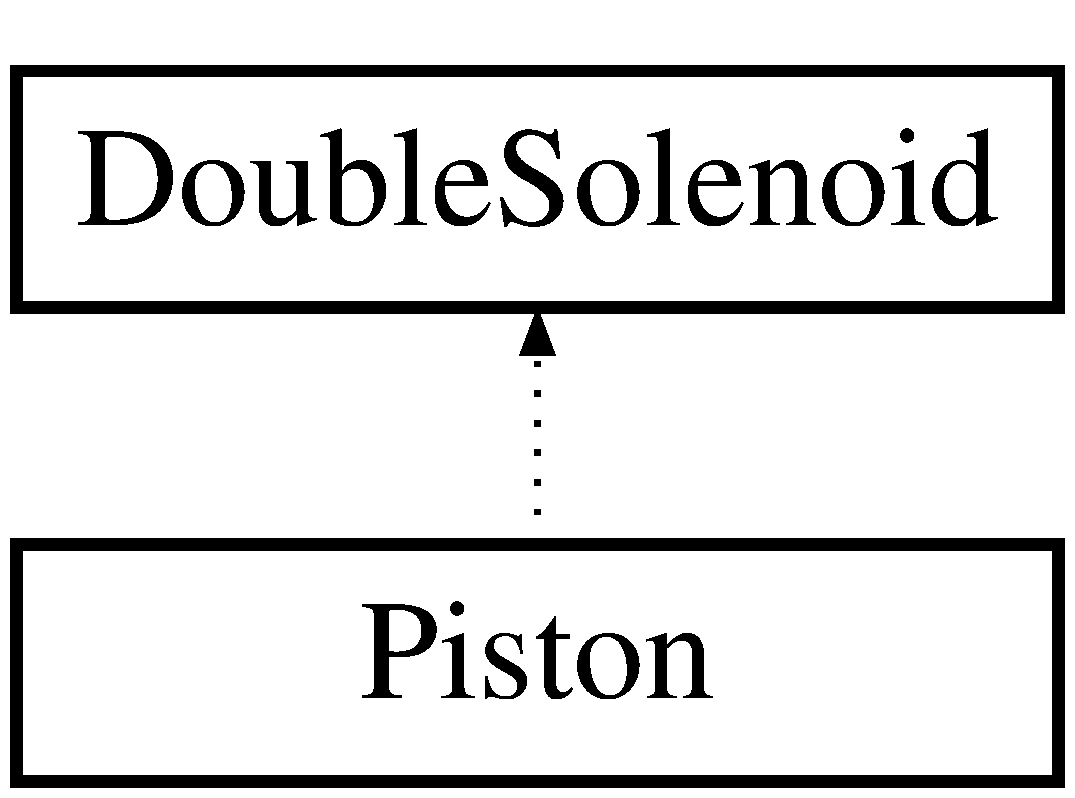
\includegraphics[height=2.000000cm]{classPiston}
\end{center}
\end{figure}
\subsection*{Public Member Functions}
\begin{DoxyCompactItemize}
\item 
\hyperlink{classPiston_abaa2dd7ebb6a1066418652aebfd62491}{Piston} (unsigned int port1, unsigned int port2)
\item 
void \hyperlink{classPiston_ad41333bdc156996df7552b766073be3d}{push\+Or\+Pull} ()
\item 
void \hyperlink{classPiston_ad02eef5cfb0ed9f92ee4605dadb46440}{Project} ()
\item 
void \hyperlink{classPiston_a37038045cb847723f935f625f4ff6d84}{Retract} ()
\item 
void \hyperlink{classPiston_a44a19e212f16a4793b125d2725c470ce}{Off} ()
\end{DoxyCompactItemize}


\subsection{Constructor \& Destructor Documentation}
\mbox{\Hypertarget{classPiston_abaa2dd7ebb6a1066418652aebfd62491}\label{classPiston_abaa2dd7ebb6a1066418652aebfd62491}} 
\index{Piston@{Piston}!Piston@{Piston}}
\index{Piston@{Piston}!Piston@{Piston}}
\subsubsection{\texorpdfstring{Piston()}{Piston()}}
{\footnotesize\ttfamily Piston\+::\+Piston (\begin{DoxyParamCaption}\item[{unsigned int}]{port1,  }\item[{unsigned int}]{port2 }\end{DoxyParamCaption})\hspace{0.3cm}{\ttfamily [inline]}}



\subsection{Member Function Documentation}
\mbox{\Hypertarget{classPiston_a44a19e212f16a4793b125d2725c470ce}\label{classPiston_a44a19e212f16a4793b125d2725c470ce}} 
\index{Piston@{Piston}!Off@{Off}}
\index{Off@{Off}!Piston@{Piston}}
\subsubsection{\texorpdfstring{Off()}{Off()}}
{\footnotesize\ttfamily void Piston\+::\+Off (\begin{DoxyParamCaption}{ }\end{DoxyParamCaption})\hspace{0.3cm}{\ttfamily [inline]}}

\mbox{\Hypertarget{classPiston_ad02eef5cfb0ed9f92ee4605dadb46440}\label{classPiston_ad02eef5cfb0ed9f92ee4605dadb46440}} 
\index{Piston@{Piston}!Project@{Project}}
\index{Project@{Project}!Piston@{Piston}}
\subsubsection{\texorpdfstring{Project()}{Project()}}
{\footnotesize\ttfamily void Piston\+::\+Project (\begin{DoxyParamCaption}{ }\end{DoxyParamCaption})\hspace{0.3cm}{\ttfamily [inline]}}

\mbox{\Hypertarget{classPiston_ad41333bdc156996df7552b766073be3d}\label{classPiston_ad41333bdc156996df7552b766073be3d}} 
\index{Piston@{Piston}!push\+Or\+Pull@{push\+Or\+Pull}}
\index{push\+Or\+Pull@{push\+Or\+Pull}!Piston@{Piston}}
\subsubsection{\texorpdfstring{push\+Or\+Pull()}{pushOrPull()}}
{\footnotesize\ttfamily void Piston\+::push\+Or\+Pull (\begin{DoxyParamCaption}{ }\end{DoxyParamCaption})\hspace{0.3cm}{\ttfamily [inline]}}

\mbox{\Hypertarget{classPiston_a37038045cb847723f935f625f4ff6d84}\label{classPiston_a37038045cb847723f935f625f4ff6d84}} 
\index{Piston@{Piston}!Retract@{Retract}}
\index{Retract@{Retract}!Piston@{Piston}}
\subsubsection{\texorpdfstring{Retract()}{Retract()}}
{\footnotesize\ttfamily void Piston\+::\+Retract (\begin{DoxyParamCaption}{ }\end{DoxyParamCaption})\hspace{0.3cm}{\ttfamily [inline]}}



The documentation for this class was generated from the following file\+:\begin{DoxyCompactItemize}
\item 
src/main/\+Utilities/\hyperlink{Piston_8h}{Piston.\+h}\end{DoxyCompactItemize}

\hypertarget{classRobot}{}\section{Robot Class Reference}
\label{classRobot}\index{Robot@{Robot}}


{\ttfamily \#include $<$Robot.\+h$>$}

Inheritance diagram for Robot\+:\begin{figure}[H]
\begin{center}
\leavevmode
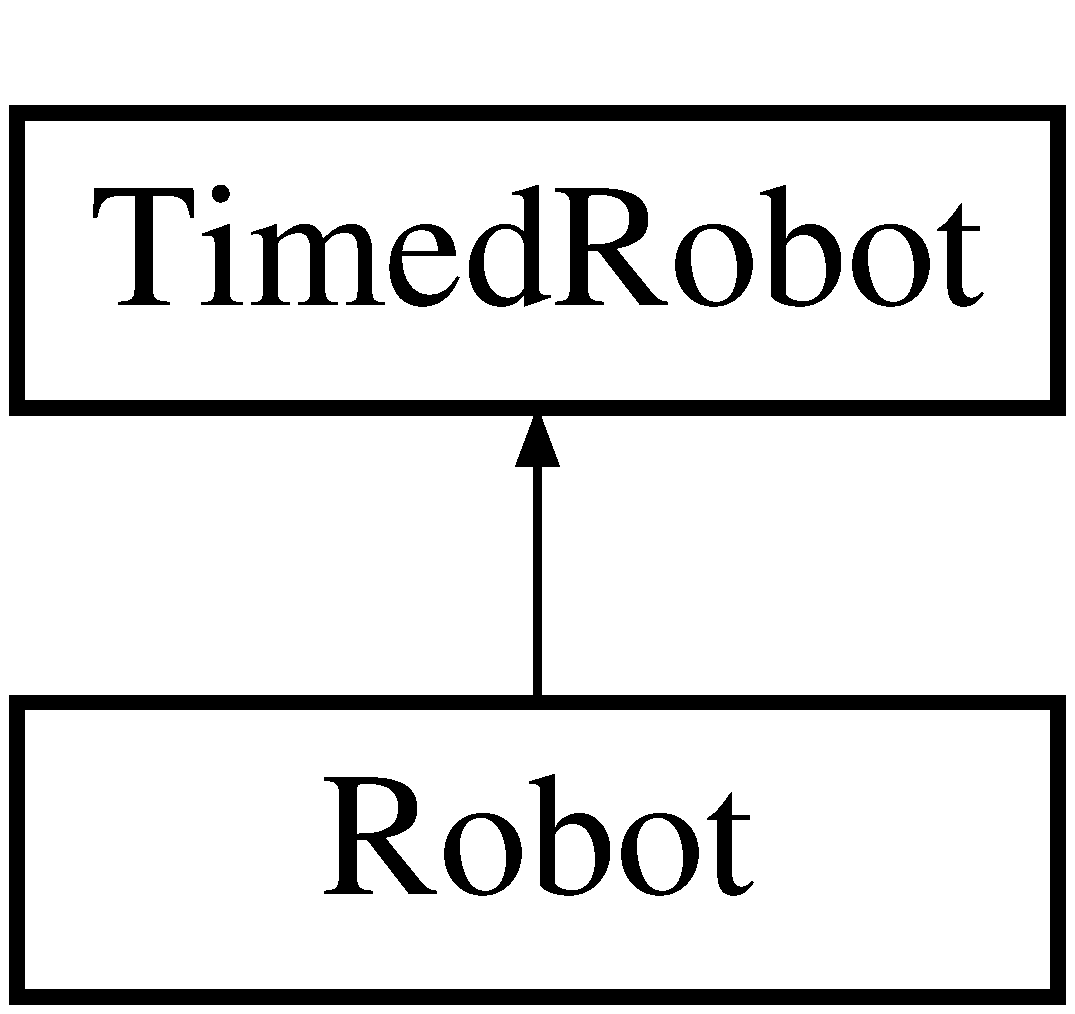
\includegraphics[height=2.000000cm]{classRobot}
\end{center}
\end{figure}
\subsection*{Public Member Functions}
\begin{DoxyCompactItemize}
\item 
void \hyperlink{classRobot_a66f23dae271748d525cf3ab046375f79}{Robot\+Init} () override
\item 
void \hyperlink{classRobot_a2136cfc015936285218c8a8db984d6bc}{Autonomous\+Init} () override
\item 
void \hyperlink{classRobot_ac11143dd674e0e02fef5329e2df24830}{Autonomous\+Periodic} () override
\item 
void \hyperlink{classRobot_aa3e246794bfbbb4406fc87f351762038}{Teleop\+Init} () override
\item 
void \hyperlink{classRobot_a324322627c63b3870daf7c7ddc5bea63}{Teleop\+Periodic} () override
\item 
void \hyperlink{classRobot_a9ac222d45d30a6d0c572fd36d18c6ccc}{Test\+Init} () override
\item 
void \hyperlink{classRobot_af0ac44a962e609e9b042285e699d1db8}{Test\+Periodic} () override
\end{DoxyCompactItemize}


\subsection{Member Function Documentation}
\mbox{\Hypertarget{classRobot_a2136cfc015936285218c8a8db984d6bc}\label{classRobot_a2136cfc015936285218c8a8db984d6bc}} 
\index{Robot@{Robot}!Autonomous\+Init@{Autonomous\+Init}}
\index{Autonomous\+Init@{Autonomous\+Init}!Robot@{Robot}}
\subsubsection{\texorpdfstring{Autonomous\+Init()}{AutonomousInit()}}
{\footnotesize\ttfamily void Robot\+::\+Autonomous\+Init (\begin{DoxyParamCaption}{ }\end{DoxyParamCaption})\hspace{0.3cm}{\ttfamily [override]}}

\mbox{\Hypertarget{classRobot_ac11143dd674e0e02fef5329e2df24830}\label{classRobot_ac11143dd674e0e02fef5329e2df24830}} 
\index{Robot@{Robot}!Autonomous\+Periodic@{Autonomous\+Periodic}}
\index{Autonomous\+Periodic@{Autonomous\+Periodic}!Robot@{Robot}}
\subsubsection{\texorpdfstring{Autonomous\+Periodic()}{AutonomousPeriodic()}}
{\footnotesize\ttfamily void Robot\+::\+Autonomous\+Periodic (\begin{DoxyParamCaption}{ }\end{DoxyParamCaption})\hspace{0.3cm}{\ttfamily [override]}}

\mbox{\Hypertarget{classRobot_a66f23dae271748d525cf3ab046375f79}\label{classRobot_a66f23dae271748d525cf3ab046375f79}} 
\index{Robot@{Robot}!Robot\+Init@{Robot\+Init}}
\index{Robot\+Init@{Robot\+Init}!Robot@{Robot}}
\subsubsection{\texorpdfstring{Robot\+Init()}{RobotInit()}}
{\footnotesize\ttfamily void Robot\+::\+Robot\+Init (\begin{DoxyParamCaption}{ }\end{DoxyParamCaption})\hspace{0.3cm}{\ttfamily [override]}}

\mbox{\Hypertarget{classRobot_aa3e246794bfbbb4406fc87f351762038}\label{classRobot_aa3e246794bfbbb4406fc87f351762038}} 
\index{Robot@{Robot}!Teleop\+Init@{Teleop\+Init}}
\index{Teleop\+Init@{Teleop\+Init}!Robot@{Robot}}
\subsubsection{\texorpdfstring{Teleop\+Init()}{TeleopInit()}}
{\footnotesize\ttfamily void Robot\+::\+Teleop\+Init (\begin{DoxyParamCaption}{ }\end{DoxyParamCaption})\hspace{0.3cm}{\ttfamily [override]}}

\mbox{\Hypertarget{classRobot_a324322627c63b3870daf7c7ddc5bea63}\label{classRobot_a324322627c63b3870daf7c7ddc5bea63}} 
\index{Robot@{Robot}!Teleop\+Periodic@{Teleop\+Periodic}}
\index{Teleop\+Periodic@{Teleop\+Periodic}!Robot@{Robot}}
\subsubsection{\texorpdfstring{Teleop\+Periodic()}{TeleopPeriodic()}}
{\footnotesize\ttfamily void Robot\+::\+Teleop\+Periodic (\begin{DoxyParamCaption}{ }\end{DoxyParamCaption})\hspace{0.3cm}{\ttfamily [override]}}

\mbox{\Hypertarget{classRobot_a9ac222d45d30a6d0c572fd36d18c6ccc}\label{classRobot_a9ac222d45d30a6d0c572fd36d18c6ccc}} 
\index{Robot@{Robot}!Test\+Init@{Test\+Init}}
\index{Test\+Init@{Test\+Init}!Robot@{Robot}}
\subsubsection{\texorpdfstring{Test\+Init()}{TestInit()}}
{\footnotesize\ttfamily void Robot\+::\+Test\+Init (\begin{DoxyParamCaption}{ }\end{DoxyParamCaption})\hspace{0.3cm}{\ttfamily [override]}}

\mbox{\Hypertarget{classRobot_af0ac44a962e609e9b042285e699d1db8}\label{classRobot_af0ac44a962e609e9b042285e699d1db8}} 
\index{Robot@{Robot}!Test\+Periodic@{Test\+Periodic}}
\index{Test\+Periodic@{Test\+Periodic}!Robot@{Robot}}
\subsubsection{\texorpdfstring{Test\+Periodic()}{TestPeriodic()}}
{\footnotesize\ttfamily void Robot\+::\+Test\+Periodic (\begin{DoxyParamCaption}{ }\end{DoxyParamCaption})\hspace{0.3cm}{\ttfamily [override]}}



The documentation for this class was generated from the following file\+:\begin{DoxyCompactItemize}
\item 
src/main/include/\hyperlink{Robot_8h}{Robot.\+h}\end{DoxyCompactItemize}

\hypertarget{classSubsystemManager}{}\section{Subsystem\+Manager Class Reference}
\label{classSubsystemManager}\index{Subsystem\+Manager@{Subsystem\+Manager}}


{\ttfamily \#include $<$Subsystem\+Manager.\+h$>$}

\subsection*{Public Member Functions}
\begin{DoxyCompactItemize}
\item 
void \hyperlink{classSubsystemManager_ae3910a93d2d417e07013d4b396d3a78b}{add\+Subsystem} (const std\+::shared\+\_\+ptr$<$ \hyperlink{classFluxSubsystem}{Flux\+Subsystem} $>$ \&new\+Sys)
\item 
void \hyperlink{classSubsystemManager_a5007405566ad61ec3a4198d81eb6edf0}{robot\+Init} ()
\item 
void \hyperlink{classSubsystemManager_a57f64def0b021ce8901cf1dfe1046256}{robot\+Update} ()
\item 
void \hyperlink{classSubsystemManager_a78e19880c05e4e2219bb5b8cf40607da}{teleop\+Init} ()
\item 
void \hyperlink{classSubsystemManager_ac55642f09846465e4482af14d835d98e}{teleop\+Update} ()
\item 
void \hyperlink{classSubsystemManager_a41232e2fb8956d8321522a23a1f63491}{auton\+Init} ()
\item 
void \hyperlink{classSubsystemManager_aa5bfa5743a4b8fdb8a6d83208b2f95dd}{auton\+Update} ()
\item 
void \hyperlink{classSubsystemManager_ac8f796d38c36f76798e992d1b1e3baef}{disable\+Init} ()
\item 
void \hyperlink{classSubsystemManager_a1c7c92c55c60928d08eec651074e74e2}{disable\+Update} ()
\end{DoxyCompactItemize}
\subsection*{Static Public Member Functions}
\begin{DoxyCompactItemize}
\item 
static \hyperlink{classSubsystemManager}{Subsystem\+Manager} \& \hyperlink{classSubsystemManager_a3acce674e15d2534ed8a0877b78ac64d}{get\+Instance} ()
\end{DoxyCompactItemize}


\subsection{Member Function Documentation}
\mbox{\Hypertarget{classSubsystemManager_ae3910a93d2d417e07013d4b396d3a78b}\label{classSubsystemManager_ae3910a93d2d417e07013d4b396d3a78b}} 
\index{Subsystem\+Manager@{Subsystem\+Manager}!add\+Subsystem@{add\+Subsystem}}
\index{add\+Subsystem@{add\+Subsystem}!Subsystem\+Manager@{Subsystem\+Manager}}
\subsubsection{\texorpdfstring{add\+Subsystem()}{addSubsystem()}}
{\footnotesize\ttfamily void Subsystem\+Manager\+::add\+Subsystem (\begin{DoxyParamCaption}\item[{const std\+::shared\+\_\+ptr$<$ \hyperlink{classFluxSubsystem}{Flux\+Subsystem} $>$ \&}]{new\+Sys }\end{DoxyParamCaption})}

Adds a subsystem to the queue, respective function of subsystem will be executed \mbox{\Hypertarget{classSubsystemManager_a41232e2fb8956d8321522a23a1f63491}\label{classSubsystemManager_a41232e2fb8956d8321522a23a1f63491}} 
\index{Subsystem\+Manager@{Subsystem\+Manager}!auton\+Init@{auton\+Init}}
\index{auton\+Init@{auton\+Init}!Subsystem\+Manager@{Subsystem\+Manager}}
\subsubsection{\texorpdfstring{auton\+Init()}{autonInit()}}
{\footnotesize\ttfamily void Subsystem\+Manager\+::auton\+Init (\begin{DoxyParamCaption}{ }\end{DoxyParamCaption})}

\mbox{\Hypertarget{classSubsystemManager_aa5bfa5743a4b8fdb8a6d83208b2f95dd}\label{classSubsystemManager_aa5bfa5743a4b8fdb8a6d83208b2f95dd}} 
\index{Subsystem\+Manager@{Subsystem\+Manager}!auton\+Update@{auton\+Update}}
\index{auton\+Update@{auton\+Update}!Subsystem\+Manager@{Subsystem\+Manager}}
\subsubsection{\texorpdfstring{auton\+Update()}{autonUpdate()}}
{\footnotesize\ttfamily void Subsystem\+Manager\+::auton\+Update (\begin{DoxyParamCaption}{ }\end{DoxyParamCaption})}

\mbox{\Hypertarget{classSubsystemManager_ac8f796d38c36f76798e992d1b1e3baef}\label{classSubsystemManager_ac8f796d38c36f76798e992d1b1e3baef}} 
\index{Subsystem\+Manager@{Subsystem\+Manager}!disable\+Init@{disable\+Init}}
\index{disable\+Init@{disable\+Init}!Subsystem\+Manager@{Subsystem\+Manager}}
\subsubsection{\texorpdfstring{disable\+Init()}{disableInit()}}
{\footnotesize\ttfamily void Subsystem\+Manager\+::disable\+Init (\begin{DoxyParamCaption}{ }\end{DoxyParamCaption})}

\mbox{\Hypertarget{classSubsystemManager_a1c7c92c55c60928d08eec651074e74e2}\label{classSubsystemManager_a1c7c92c55c60928d08eec651074e74e2}} 
\index{Subsystem\+Manager@{Subsystem\+Manager}!disable\+Update@{disable\+Update}}
\index{disable\+Update@{disable\+Update}!Subsystem\+Manager@{Subsystem\+Manager}}
\subsubsection{\texorpdfstring{disable\+Update()}{disableUpdate()}}
{\footnotesize\ttfamily void Subsystem\+Manager\+::disable\+Update (\begin{DoxyParamCaption}{ }\end{DoxyParamCaption})}

\mbox{\Hypertarget{classSubsystemManager_a3acce674e15d2534ed8a0877b78ac64d}\label{classSubsystemManager_a3acce674e15d2534ed8a0877b78ac64d}} 
\index{Subsystem\+Manager@{Subsystem\+Manager}!get\+Instance@{get\+Instance}}
\index{get\+Instance@{get\+Instance}!Subsystem\+Manager@{Subsystem\+Manager}}
\subsubsection{\texorpdfstring{get\+Instance()}{getInstance()}}
{\footnotesize\ttfamily static \hyperlink{classSubsystemManager}{Subsystem\+Manager}\& Subsystem\+Manager\+::get\+Instance (\begin{DoxyParamCaption}{ }\end{DoxyParamCaption})\hspace{0.3cm}{\ttfamily [inline]}, {\ttfamily [static]}}

\mbox{\Hypertarget{classSubsystemManager_a5007405566ad61ec3a4198d81eb6edf0}\label{classSubsystemManager_a5007405566ad61ec3a4198d81eb6edf0}} 
\index{Subsystem\+Manager@{Subsystem\+Manager}!robot\+Init@{robot\+Init}}
\index{robot\+Init@{robot\+Init}!Subsystem\+Manager@{Subsystem\+Manager}}
\subsubsection{\texorpdfstring{robot\+Init()}{robotInit()}}
{\footnotesize\ttfamily void Subsystem\+Manager\+::robot\+Init (\begin{DoxyParamCaption}{ }\end{DoxyParamCaption})}

\mbox{\Hypertarget{classSubsystemManager_a57f64def0b021ce8901cf1dfe1046256}\label{classSubsystemManager_a57f64def0b021ce8901cf1dfe1046256}} 
\index{Subsystem\+Manager@{Subsystem\+Manager}!robot\+Update@{robot\+Update}}
\index{robot\+Update@{robot\+Update}!Subsystem\+Manager@{Subsystem\+Manager}}
\subsubsection{\texorpdfstring{robot\+Update()}{robotUpdate()}}
{\footnotesize\ttfamily void Subsystem\+Manager\+::robot\+Update (\begin{DoxyParamCaption}{ }\end{DoxyParamCaption})}

\mbox{\Hypertarget{classSubsystemManager_a78e19880c05e4e2219bb5b8cf40607da}\label{classSubsystemManager_a78e19880c05e4e2219bb5b8cf40607da}} 
\index{Subsystem\+Manager@{Subsystem\+Manager}!teleop\+Init@{teleop\+Init}}
\index{teleop\+Init@{teleop\+Init}!Subsystem\+Manager@{Subsystem\+Manager}}
\subsubsection{\texorpdfstring{teleop\+Init()}{teleopInit()}}
{\footnotesize\ttfamily void Subsystem\+Manager\+::teleop\+Init (\begin{DoxyParamCaption}{ }\end{DoxyParamCaption})}

\mbox{\Hypertarget{classSubsystemManager_ac55642f09846465e4482af14d835d98e}\label{classSubsystemManager_ac55642f09846465e4482af14d835d98e}} 
\index{Subsystem\+Manager@{Subsystem\+Manager}!teleop\+Update@{teleop\+Update}}
\index{teleop\+Update@{teleop\+Update}!Subsystem\+Manager@{Subsystem\+Manager}}
\subsubsection{\texorpdfstring{teleop\+Update()}{teleopUpdate()}}
{\footnotesize\ttfamily void Subsystem\+Manager\+::teleop\+Update (\begin{DoxyParamCaption}{ }\end{DoxyParamCaption})}



The documentation for this class was generated from the following files\+:\begin{DoxyCompactItemize}
\item 
src/main/\+Subsystems/\hyperlink{SubsystemManager_8h}{Subsystem\+Manager.\+h}\item 
src/main/\+Subsystems/\hyperlink{SubsystemManager_8cpp}{Subsystem\+Manager.\+cpp}\end{DoxyCompactItemize}

\chapter{File Documentation}
\hypertarget{BasicChassis_8h}{}\section{src/main/2019/\+Mechs/\+Basic\+Chassis.h File Reference}
\label{BasicChassis_8h}\index{src/main/2019/\+Mechs/\+Basic\+Chassis.\+h@{src/main/2019/\+Mechs/\+Basic\+Chassis.\+h}}
{\ttfamily \#include \char`\"{}Subsystems/\+Flux\+Subsystem.\+h\char`\"{}}\newline

\hypertarget{CargoPod_8cpp}{}\section{src/main/2019/\+Mechs/\+Cargo\+Pod.cpp File Reference}
\label{CargoPod_8cpp}\index{src/main/2019/\+Mechs/\+Cargo\+Pod.\+cpp@{src/main/2019/\+Mechs/\+Cargo\+Pod.\+cpp}}
{\ttfamily \#include \char`\"{}2019/\+Mechs/\+Cargo\+Pod.\+h\char`\"{}}\newline

\hypertarget{CargoPod_8h}{}\section{src/main/2019/\+Mechs/\+Cargo\+Pod.h File Reference}
\label{CargoPod_8h}\index{src/main/2019/\+Mechs/\+Cargo\+Pod.\+h@{src/main/2019/\+Mechs/\+Cargo\+Pod.\+h}}
{\ttfamily \#include \char`\"{}Subsystems/\+Flux\+Subsystem.\+h\char`\"{}}\newline
{\ttfamily \#include \char`\"{}Utilities/\+Flux\+Victor.\+h\char`\"{}}\newline
{\ttfamily \#include \char`\"{}frc/\+Xbox\+Controller.\+h\char`\"{}}\newline
{\ttfamily \#include \char`\"{}Utilities/\+Piston.\+h\char`\"{}}\newline
{\ttfamily \#include \char`\"{}frc/\+Solenoid.\+h\char`\"{}}\newline
{\ttfamily \#include \char`\"{}frc/\+Victor\+S\+P.\+h\char`\"{}}\newline
{\ttfamily \#include \char`\"{}Subsystems/\+Datapool.\+h\char`\"{}}\newline
{\ttfamily \#include \char`\"{}frc/smartdashboard/\+Smart\+Dashboard.\+h\char`\"{}}\newline
\subsection*{Classes}
\begin{DoxyCompactItemize}
\item 
class \hyperlink{classCargoPod}{Cargo\+Pod}
\end{DoxyCompactItemize}

\hypertarget{DriveTrain_8cpp}{}\section{src/main/2019/\+Mechs/\+Drive\+Train.cpp File Reference}
\label{DriveTrain_8cpp}\index{src/main/2019/\+Mechs/\+Drive\+Train.\+cpp@{src/main/2019/\+Mechs/\+Drive\+Train.\+cpp}}
{\ttfamily \#include \char`\"{}2019/\+Mechs/\+Drive\+Train.\+h\char`\"{}}\newline

\hypertarget{DriveTrain_8h}{}\section{src/main/2019/\+Mechs/\+Drive\+Train.h File Reference}
\label{DriveTrain_8h}\index{src/main/2019/\+Mechs/\+Drive\+Train.\+h@{src/main/2019/\+Mechs/\+Drive\+Train.\+h}}
{\ttfamily \#include \char`\"{}Subsystems/\+Flux\+Subsystem.\+h\char`\"{}}\newline
{\ttfamily \#include \char`\"{}Utilities/\+Flux\+Controller.\+h\char`\"{}}\newline
{\ttfamily \#include \char`\"{}Utilities/\+Flux\+Victor.\+h\char`\"{}}\newline
\subsection*{Classes}
\begin{DoxyCompactItemize}
\item 
class \hyperlink{classDrivetrain}{Drivetrain}
\end{DoxyCompactItemize}

\hypertarget{Hatcher_8cpp}{}\section{src/main/2019/\+Mechs/\+Hatcher.cpp File Reference}
\label{Hatcher_8cpp}\index{src/main/2019/\+Mechs/\+Hatcher.\+cpp@{src/main/2019/\+Mechs/\+Hatcher.\+cpp}}
{\ttfamily \#include \char`\"{}2019/\+Mechs/\+Hatcher.\+h\char`\"{}}\newline

\hypertarget{Hatcher_8h}{}\section{src/main/2019/\+Mechs/\+Hatcher.h File Reference}
\label{Hatcher_8h}\index{src/main/2019/\+Mechs/\+Hatcher.\+h@{src/main/2019/\+Mechs/\+Hatcher.\+h}}
{\ttfamily \#include \char`\"{}Utilities/\+Piston.\+h\char`\"{}}\newline
{\ttfamily \#include \char`\"{}Subsystems/\+Flux\+Subsystem.\+h\char`\"{}}\newline
{\ttfamily \#include \char`\"{}frc/\+Xbox\+Controller.\+h\char`\"{}}\newline
\subsection*{Classes}
\begin{DoxyCompactItemize}
\item 
class \hyperlink{classHatcher}{Hatcher}
\end{DoxyCompactItemize}

\hypertarget{Pepochassis_8cpp}{}\section{src/main/2019/\+Pepito/\+Mechs/\+Pepochassis.cpp File Reference}
\label{Pepochassis_8cpp}\index{src/main/2019/\+Pepito/\+Mechs/\+Pepochassis.\+cpp@{src/main/2019/\+Pepito/\+Mechs/\+Pepochassis.\+cpp}}
{\ttfamily \#include \char`\"{}2019/\+Pepito/\+Mechs/\+Pepochassis.\+h\char`\"{}}\newline

\hypertarget{Pepochassis_8h}{}\section{src/main/2019/\+Pepito/\+Mechs/\+Pepochassis.h File Reference}
\label{Pepochassis_8h}\index{src/main/2019/\+Pepito/\+Mechs/\+Pepochassis.\+h@{src/main/2019/\+Pepito/\+Mechs/\+Pepochassis.\+h}}
{\ttfamily \#include \char`\"{}Subsystems/\+Flux\+Subsystem.\+h\char`\"{}}\newline
{\ttfamily \#include \char`\"{}ctre/\+Phoenix.\+h\char`\"{}}\newline
{\ttfamily \#include \char`\"{}frc/smartdashboard/\+Smart\+Dashboard.\+h\char`\"{}}\newline
{\ttfamily \#include $<$cmath$>$}\newline
{\ttfamily \#include \char`\"{}frc/\+Xbox\+Controller.\+h\char`\"{}}\newline
{\ttfamily \#include \char`\"{}frc/\+A\+D\+X\+R\+S450\+\_\+\+Gyro.\+h\char`\"{}}\newline
{\ttfamily \#include \char`\"{}Subsystems/\+Datapool.\+h\char`\"{}}\newline
{\ttfamily \#include \char`\"{}frc/\+Victor\+S\+P.\+h\char`\"{}}\newline
{\ttfamily \#include \char`\"{}Utilities/\+Piston.\+h\char`\"{}}\newline
{\ttfamily \#include \char`\"{}Utilities/\+Flux\+Controller.\+h\char`\"{}}\newline
{\ttfamily \#include \char`\"{}Sensors/\+Flux\+R\+S450.\+h\char`\"{}}\newline
{\ttfamily \#include \char`\"{}Utilities/\+Flux\+Victor.\+h\char`\"{}}\newline
{\ttfamily \#include $<$cameraserver/\+Camera\+Server.\+h$>$}\newline
{\ttfamily \#include $<$wpi/raw\+\_\+ostream.\+h$>$}\newline
{\ttfamily \#include \char`\"{}networktables/\+Network\+Table\+Instance.\+h\char`\"{}}\newline
{\ttfamily \#include $<$chrono$>$}\newline
\subsection*{Classes}
\begin{DoxyCompactItemize}
\item 
class \hyperlink{classPepoChassis}{Pepo\+Chassis}
\end{DoxyCompactItemize}

\hypertarget{Pepito_8cpp}{}\section{src/main/2019/\+Pepito/\+Pepito.cpp File Reference}
\label{Pepito_8cpp}\index{src/main/2019/\+Pepito/\+Pepito.\+cpp@{src/main/2019/\+Pepito/\+Pepito.\+cpp}}
{\ttfamily \#include \char`\"{}2019/\+Pepito/\+Pepito.\+h\char`\"{}}\newline
{\ttfamily \#include \char`\"{}2019/\+Mechs/\+Cargo\+Pod.\+h\char`\"{}}\newline
{\ttfamily \#include \char`\"{}2019/\+Mechs/\+Hatcher.\+h\char`\"{}}\newline

\hypertarget{Pepito_8h}{}\section{src/main/2019/\+Pepito/\+Pepito.h File Reference}
\label{Pepito_8h}\index{src/main/2019/\+Pepito/\+Pepito.\+h@{src/main/2019/\+Pepito/\+Pepito.\+h}}
{\ttfamily \#include $<$iostream$>$}\newline
{\ttfamily \#include \char`\"{}Subsystems/\+Flux\+Robot.\+h\char`\"{}}\newline
{\ttfamily \#include \char`\"{}2019/\+Pepito/\+Mechs/\+Pepochassis.\+h\char`\"{}}\newline
\subsection*{Classes}
\begin{DoxyCompactItemize}
\item 
class \hyperlink{classPepito}{Pepito}
\end{DoxyCompactItemize}

\hypertarget{Delorean_8cpp}{}\section{src/main/2019/\+Robots/\+Delorean.cpp File Reference}
\label{Delorean_8cpp}\index{src/main/2019/\+Robots/\+Delorean.\+cpp@{src/main/2019/\+Robots/\+Delorean.\+cpp}}
{\ttfamily \#include \char`\"{}2019/\+Robots/\+Delorean.\+h\char`\"{}}\newline

\hypertarget{Delorean_8h}{}\section{src/main/2019/\+Robots/\+Delorean.h File Reference}
\label{Delorean_8h}\index{src/main/2019/\+Robots/\+Delorean.\+h@{src/main/2019/\+Robots/\+Delorean.\+h}}
{\ttfamily \#include $<$iostream$>$}\newline
{\ttfamily \#include \char`\"{}Subsystems/\+Flux\+Robot.\+h\char`\"{}}\newline
{\ttfamily \#include \char`\"{}Subsystems/\+Flux\+Chassis.\+h\char`\"{}}\newline
{\ttfamily \#include \char`\"{}2019/\+Mechs/\+Cargo\+Pod.\+h\char`\"{}}\newline
{\ttfamily \#include \char`\"{}2019/\+Mechs/\+Hatcher.\+h\char`\"{}}\newline
\subsection*{Classes}
\begin{DoxyCompactItemize}
\item 
class \hyperlink{classDelorean}{Delorean}
\end{DoxyCompactItemize}

\hypertarget{Robot_8h}{}\section{src/main/include/\+Robot.h File Reference}
\label{Robot_8h}\index{src/main/include/\+Robot.\+h@{src/main/include/\+Robot.\+h}}
{\ttfamily \#include $<$frc/\+Timed\+Robot.\+h$>$}\newline
\subsection*{Classes}
\begin{DoxyCompactItemize}
\item 
class \hyperlink{classRobot}{Robot}
\end{DoxyCompactItemize}

\hypertarget{main_2main_8cpp}{}\section{src/main/main.cpp File Reference}
\label{main_2main_8cpp}\index{src/main/main.\+cpp@{src/main/main.\+cpp}}
{\ttfamily \#include \char`\"{}2019/\+Robots/\+Delorean.\+h\char`\"{}}\newline
{\ttfamily \#include \char`\"{}2019/\+Pepito/\+Pepito.\+h\char`\"{}}\newline
\subsection*{Functions}
\begin{DoxyCompactItemize}
\item 
int \hyperlink{main_2main_8cpp_ae66f6b31b5ad750f1fe042a706a4e3d4}{main} ()
\end{DoxyCompactItemize}


\subsection{Function Documentation}
\mbox{\Hypertarget{main_2main_8cpp_ae66f6b31b5ad750f1fe042a706a4e3d4}\label{main_2main_8cpp_ae66f6b31b5ad750f1fe042a706a4e3d4}} 
\index{main/main.\+cpp@{main/main.\+cpp}!main@{main}}
\index{main@{main}!main/main.\+cpp@{main/main.\+cpp}}
\subsubsection{\texorpdfstring{main()}{main()}}
{\footnotesize\ttfamily int main (\begin{DoxyParamCaption}{ }\end{DoxyParamCaption})}


\hypertarget{test_2cpp_2main_8cpp}{}\section{src/test/cpp/main.cpp File Reference}
\label{test_2cpp_2main_8cpp}\index{src/test/cpp/main.\+cpp@{src/test/cpp/main.\+cpp}}
{\ttfamily \#include $<$hal/\+H\+A\+L.\+h$>$}\newline
{\ttfamily \#include \char`\"{}gtest/gtest.\+h\char`\"{}}\newline
\subsection*{Functions}
\begin{DoxyCompactItemize}
\item 
int \hyperlink{test_2cpp_2main_8cpp_a3c04138a5bfe5d72780bb7e82a18e627}{main} (int argc, char $\ast$$\ast$argv)
\end{DoxyCompactItemize}


\subsection{Function Documentation}
\mbox{\Hypertarget{test_2cpp_2main_8cpp_a3c04138a5bfe5d72780bb7e82a18e627}\label{test_2cpp_2main_8cpp_a3c04138a5bfe5d72780bb7e82a18e627}} 
\index{test/cpp/main.\+cpp@{test/cpp/main.\+cpp}!main@{main}}
\index{main@{main}!test/cpp/main.\+cpp@{test/cpp/main.\+cpp}}
\subsubsection{\texorpdfstring{main()}{main()}}
{\footnotesize\ttfamily int main (\begin{DoxyParamCaption}\item[{int}]{argc,  }\item[{char $\ast$$\ast$}]{argv }\end{DoxyParamCaption})}


\hypertarget{FluxRS450_8cpp}{}\section{src/main/\+Sensors/\+Flux\+R\+S450.cpp File Reference}
\label{FluxRS450_8cpp}\index{src/main/\+Sensors/\+Flux\+R\+S450.\+cpp@{src/main/\+Sensors/\+Flux\+R\+S450.\+cpp}}
{\ttfamily \#include \char`\"{}Sensors/\+Flux\+R\+S450.\+h\char`\"{}}\newline

\hypertarget{FluxRS450_8h}{}\section{src/main/\+Sensors/\+Flux\+R\+S450.h File Reference}
\label{FluxRS450_8h}\index{src/main/\+Sensors/\+Flux\+R\+S450.\+h@{src/main/\+Sensors/\+Flux\+R\+S450.\+h}}
{\ttfamily \#include \char`\"{}frc/\+A\+D\+X\+R\+S450\+\_\+\+Gyro.\+h\char`\"{}}\newline
\subsection*{Classes}
\begin{DoxyCompactItemize}
\item 
class \hyperlink{classFluxRS450}{Flux\+R\+S450}
\end{DoxyCompactItemize}

\hypertarget{Odometry_8h}{}\section{src/main/\+Sensors/\+Odometry.h File Reference}
\label{Odometry_8h}\index{src/main/\+Sensors/\+Odometry.\+h@{src/main/\+Sensors/\+Odometry.\+h}}
{\ttfamily \#include \char`\"{}frc/\+Encoder.\+h\char`\"{}}\newline
{\ttfamily \#include \char`\"{}Subsystems/\+Flux\+Subsystem.\+h\char`\"{}}\newline
{\ttfamily \#include \char`\"{}Subsystems/\+Datapool.\+h\char`\"{}}\newline
\subsection*{Classes}
\begin{DoxyCompactItemize}
\item 
class \hyperlink{classOdometry}{Odometry}
\end{DoxyCompactItemize}

\hypertarget{Datapool_8cpp}{}\section{src/main/\+Subsystems/\+Datapool.cpp File Reference}
\label{Datapool_8cpp}\index{src/main/\+Subsystems/\+Datapool.\+cpp@{src/main/\+Subsystems/\+Datapool.\+cpp}}
{\ttfamily \#include \char`\"{}Subsystems/\+Datapool.\+h\char`\"{}}\newline

\hypertarget{Datapool_8h}{}\section{src/main/\+Subsystems/\+Datapool.h File Reference}
\label{Datapool_8h}\index{src/main/\+Subsystems/\+Datapool.\+h@{src/main/\+Subsystems/\+Datapool.\+h}}
{\ttfamily \#include $<$string$>$}\newline
{\ttfamily \#include $<$iostream$>$}\newline
{\ttfamily \#include $<$map$>$}\newline
\subsection*{Classes}
\begin{DoxyCompactItemize}
\item 
class \hyperlink{classDatapool}{Datapool}
\end{DoxyCompactItemize}

\hypertarget{FluxRobot_8cpp}{}\section{src/main/\+Subsystems/\+Flux\+Robot.cpp File Reference}
\label{FluxRobot_8cpp}\index{src/main/\+Subsystems/\+Flux\+Robot.\+cpp@{src/main/\+Subsystems/\+Flux\+Robot.\+cpp}}
{\ttfamily \#include \char`\"{}Subsystems/\+Flux\+Robot.\+h\char`\"{}}\newline

\hypertarget{FluxRobot_8h}{}\section{src/main/\+Subsystems/\+Flux\+Robot.h File Reference}
\label{FluxRobot_8h}\index{src/main/\+Subsystems/\+Flux\+Robot.\+h@{src/main/\+Subsystems/\+Flux\+Robot.\+h}}
{\ttfamily \#include \char`\"{}frc/\+W\+P\+I\+Lib.\+h\char`\"{}}\newline
{\ttfamily \#include \char`\"{}Subsystems/\+Flux\+Subsystem.\+h\char`\"{}}\newline
{\ttfamily \#include \char`\"{}Subsystems/\+Subsystem\+Manager.\+h\char`\"{}}\newline
{\ttfamily \#include $<$string$>$}\newline
\subsection*{Classes}
\begin{DoxyCompactItemize}
\item 
class \hyperlink{classFluxRobot}{Flux\+Robot}
\end{DoxyCompactItemize}

\hypertarget{FluxSubsystem_8cpp}{}\section{src/main/\+Subsystems/\+Flux\+Subsystem.cpp File Reference}
\label{FluxSubsystem_8cpp}\index{src/main/\+Subsystems/\+Flux\+Subsystem.\+cpp@{src/main/\+Subsystems/\+Flux\+Subsystem.\+cpp}}
{\ttfamily \#include \char`\"{}Subsystems/\+Flux\+Subsystem.\+h\char`\"{}}\newline

\hypertarget{FluxSubsystem_8h}{}\section{src/main/\+Subsystems/\+Flux\+Subsystem.h File Reference}
\label{FluxSubsystem_8h}\index{src/main/\+Subsystems/\+Flux\+Subsystem.\+h@{src/main/\+Subsystems/\+Flux\+Subsystem.\+h}}
{\ttfamily \#include $<$string$>$}\newline
{\ttfamily \#include $<$memory$>$}\newline
\subsection*{Classes}
\begin{DoxyCompactItemize}
\item 
class \hyperlink{classFluxSubsystem}{Flux\+Subsystem}
\end{DoxyCompactItemize}

\hypertarget{SubsystemManager_8cpp}{}\section{src/main/\+Subsystems/\+Subsystem\+Manager.cpp File Reference}
\label{SubsystemManager_8cpp}\index{src/main/\+Subsystems/\+Subsystem\+Manager.\+cpp@{src/main/\+Subsystems/\+Subsystem\+Manager.\+cpp}}
{\ttfamily \#include \char`\"{}Subsystems/\+Subsystem\+Manager.\+h\char`\"{}}\newline
{\ttfamily \#include $<$frc/\+Timer.\+h$>$}\newline

\hypertarget{SubsystemManager_8h}{}\section{src/main/\+Subsystems/\+Subsystem\+Manager.h File Reference}
\label{SubsystemManager_8h}\index{src/main/\+Subsystems/\+Subsystem\+Manager.\+h@{src/main/\+Subsystems/\+Subsystem\+Manager.\+h}}
{\ttfamily \#include \char`\"{}Subsystems/\+Flux\+Subsystem.\+h\char`\"{}}\newline
{\ttfamily \#include $<$memory$>$}\newline
{\ttfamily \#include $<$vector$>$}\newline
\subsection*{Classes}
\begin{DoxyCompactItemize}
\item 
class \hyperlink{classSubsystemManager}{Subsystem\+Manager}
\end{DoxyCompactItemize}

\hypertarget{FluxController_8cpp}{}\section{src/main/\+Utilities/\+Flux\+Controller.cpp File Reference}
\label{FluxController_8cpp}\index{src/main/\+Utilities/\+Flux\+Controller.\+cpp@{src/main/\+Utilities/\+Flux\+Controller.\+cpp}}
{\ttfamily \#include \char`\"{}Utilities/\+Flux\+Controller.\+h\char`\"{}}\newline

\hypertarget{FluxController_8h}{}\section{src/main/\+Utilities/\+Flux\+Controller.h File Reference}
\label{FluxController_8h}\index{src/main/\+Utilities/\+Flux\+Controller.\+h@{src/main/\+Utilities/\+Flux\+Controller.\+h}}
{\ttfamily \#include \char`\"{}frc/\+Xbox\+Controller.\+h\char`\"{}}\newline
\subsection*{Classes}
\begin{DoxyCompactItemize}
\item 
struct \hyperlink{structAnalogStates}{Analog\+States}
\item 
class \hyperlink{classFluxcontroller}{Fluxcontroller}
\end{DoxyCompactItemize}
\subsection*{Enumerations}
\begin{DoxyCompactItemize}
\item 
enum \hyperlink{FluxController_8h_a899b1f99e0792573e6e4b51d84f78653}{H\+A\+ND} \{ \hyperlink{FluxController_8h_a899b1f99e0792573e6e4b51d84f78653adb45120aafd37a973140edee24708065}{L\+E\+FT}, 
\hyperlink{FluxController_8h_a899b1f99e0792573e6e4b51d84f78653aec8379af7490bb9eaaf579cf17876f38}{R\+I\+G\+HT}
 \}
\end{DoxyCompactItemize}


\subsection{Enumeration Type Documentation}
\mbox{\Hypertarget{FluxController_8h_a899b1f99e0792573e6e4b51d84f78653}\label{FluxController_8h_a899b1f99e0792573e6e4b51d84f78653}} 
\index{Flux\+Controller.\+h@{Flux\+Controller.\+h}!H\+A\+ND@{H\+A\+ND}}
\index{H\+A\+ND@{H\+A\+ND}!Flux\+Controller.\+h@{Flux\+Controller.\+h}}
\subsubsection{\texorpdfstring{H\+A\+ND}{HAND}}
{\footnotesize\ttfamily enum \hyperlink{FluxController_8h_a899b1f99e0792573e6e4b51d84f78653}{H\+A\+ND}}

\begin{DoxyEnumFields}{Enumerator}
\raisebox{\heightof{T}}[0pt][0pt]{\index{L\+E\+FT@{L\+E\+FT}!Flux\+Controller.\+h@{Flux\+Controller.\+h}}\index{Flux\+Controller.\+h@{Flux\+Controller.\+h}!L\+E\+FT@{L\+E\+FT}}}\mbox{\Hypertarget{FluxController_8h_a899b1f99e0792573e6e4b51d84f78653adb45120aafd37a973140edee24708065}\label{FluxController_8h_a899b1f99e0792573e6e4b51d84f78653adb45120aafd37a973140edee24708065}} 
L\+E\+FT&\\
\hline

\raisebox{\heightof{T}}[0pt][0pt]{\index{R\+I\+G\+HT@{R\+I\+G\+HT}!Flux\+Controller.\+h@{Flux\+Controller.\+h}}\index{Flux\+Controller.\+h@{Flux\+Controller.\+h}!R\+I\+G\+HT@{R\+I\+G\+HT}}}\mbox{\Hypertarget{FluxController_8h_a899b1f99e0792573e6e4b51d84f78653aec8379af7490bb9eaaf579cf17876f38}\label{FluxController_8h_a899b1f99e0792573e6e4b51d84f78653aec8379af7490bb9eaaf579cf17876f38}} 
R\+I\+G\+HT&\\
\hline

\end{DoxyEnumFields}

\hypertarget{FluxVictor_8cpp}{}\section{src/main/\+Utilities/\+Flux\+Victor.cpp File Reference}
\label{FluxVictor_8cpp}\index{src/main/\+Utilities/\+Flux\+Victor.\+cpp@{src/main/\+Utilities/\+Flux\+Victor.\+cpp}}
{\ttfamily \#include \char`\"{}Utilities/\+Flux\+Victor.\+h\char`\"{}}\newline

\hypertarget{FluxVictor_8h}{}\section{src/main/\+Utilities/\+Flux\+Victor.h File Reference}
\label{FluxVictor_8h}\index{src/main/\+Utilities/\+Flux\+Victor.\+h@{src/main/\+Utilities/\+Flux\+Victor.\+h}}
{\ttfamily \#include \char`\"{}ctre/\+Phoenix.\+h\char`\"{}}\newline
\subsection*{Classes}
\begin{DoxyCompactItemize}
\item 
class \hyperlink{classFluxVictor}{Flux\+Victor}
\end{DoxyCompactItemize}

\hypertarget{Piston_8h}{}\section{src/main/\+Utilities/\+Piston.h File Reference}
\label{Piston_8h}\index{src/main/\+Utilities/\+Piston.\+h@{src/main/\+Utilities/\+Piston.\+h}}
{\ttfamily \#include \char`\"{}frc/\+Double\+Solenoid.\+h\char`\"{}}\newline
\subsection*{Classes}
\begin{DoxyCompactItemize}
\item 
class \hyperlink{classPiston}{Piston}
\end{DoxyCompactItemize}

%--- End generated contents ---

% Index
\backmatter
\newpage
\phantomsection
\clearemptydoublepage
\addcontentsline{toc}{chapter}{Index}
\printindex

\end{document}
